\documentclass[12pt]{article}
\usepackage{listings}
\usepackage{cite} % sort citations 
\usepackage{amsmath,xspace,../../design/aux/math-envs,../../design/aux/math-cmds,../../design/aux/code,../../design/aux/proof,stmaryrd,pifont,../../design/aux/bussproofs,fullpage}
\usepackage[pdftex]{graphicx}
\usepackage[small]{caption}
% code.sty: -*- latex -*-
% Latex macros for a "weak" verbatim mode.
% -- like verbatim, except \, {, and } have their usual meanings.

% Environments: code, tightcode,  codeaux, codebox, centercode
% Commands: \dcd, \cddollar, \cdmath, \cd, \codeallowbreaks, \codeskip, \^
% Already defined in LaTeX, but of some relevance: \#, \$, \%, \&, \_, \{, \}

% Changelog at the end of the file.

% These commands give you an environment, code, that is like verbatim
% except that you can still insert commands in the middle of the environment:
%     \begin{code}
%     for(x=1; x<loop_bound; x++)
%         y += x^3; /* {\em Add in {\tt x} cubed} */
%     \end{code}
%
% All characters are ordinary except \{}. To get \{} in your text, 
% you use the commands \\, \{, and \}.

% These macros mess with the definition of the special chars (e.g., ^_~%).
% The characters \{} are left alone, so you can still have embedded commands:
%	\begin{code} f(a,b,\ldots,y,z) \end{code}
% However, if your embedded commands use the formerly-special chars, as in
%    	\begin{code} x := x+1 /* \mbox{\em This is $y^3$} */ \end{code}
% then you lose. The $ and ^ chars are scanned in as non-specials,
% so they don't work. If the chars are scanned *outside* the code env,
% then you have no problem:
% 	\def\ycube{$y^3$}
% 	\begin{code} x := x+1 /* {\em This is \ycube} */ \end{code}
% If you must put special chars inside the code env, you do it by
% prefixing them with the special \dcd ("decode") command, that
% reverts the chars to back to special status:
%    	\begin{code} x := x+1 /* {\dcd\em This is $y^3$} */ \end{code}
% \dcd's scope is bounded by its enclosing braces. It is only defined within
% the code env. You can also turn on just $ with the \cddollar command;
% you can turn on just $^_ with the \cdmath command. See below.
%
% Alternatively, just use \(...\) for $...$, \sp for ^, and \sb for _.

% WARNING:
% Like \verb, you cannot put a \cd{...} inside an argument to a macro
% or a command. If you try, for example,
%     \mbox{\cd{$x^y$}}
% you will lose. That is because the text "\cd{$x^y$}" gets read in
% as \mbox's argument before the \cd executes. But the \cd has to
% have a chance to run before LaTeX ever reads the $x^y$ so it can
% turn off the specialness of $ and ^. So, \cd has to appear at
% top level, not inside an argument. Similarly, you can't have
% a \cd or a \code inside a macro (Although you could use \gdef to
% define a macro *inside* a \cd, which you could then use outside.
% Don't worry about this if you don't understand it.)

% BUG: In the codebox env, the effect of a \dcd, \cddollar, or \cdmath
%   command is reset at the end of each line. This can be hacked by
%   messing with the \halign's preamble, if you feel up to it.

% Useage note: the initial newline after the \begin{code} or 
%   \begin{codebox} is eaten, but the last newline is not.
%   So,
%     \begin{code}
%     foo
%     bar
%     \end{code}
%  leaves one more blank line after bar than does
%     \begin{code}
%     foo
%     bar\end{code}
%  Moral: get in the habit of terminating code envs without a newline
%  (as in the second example).
%

%
% get the paragraph indentation (use \edef and \the to force evaluation)
%
%\edef\codeindent{\the\parindent}
\edef\codeindent{0pt}


% All this stuff tweaks the meaning of space, tab, and newline.
%===============================================================================
% \cd@obeyspaces
% Turns all spaces into non-breakable spaces.
% Note: this is like \@vobeyspaces except without spurious space in defn.
% @xobeysp is basically a space; it's defined in latex.tex.
%
{\catcode`\ =\active\gdef\cd@obeyspaces{\catcode`\ =\active\let =\@xobeysp}}



% \cd@obeytabs
% Turns all tabs into 8 non-breakable spaces (which is bogus).
%
{\catcode`\^^I=\active %
  \gdef\cd@obeytabs{\catcode`\^^I=\active\let^^I=\cd@tab}}

\def\cd@tab{\@xobeysp\@xobeysp\@xobeysp\@xobeysp\@xobeysp\@xobeysp\@xobeysp\@xobeysp}



% \cd@obeylines
% Turns all cr's into linebreaks. Pagebreaks are not permitted between lines.
% This is copied from lplain.tex's \obeylines, with the cr def'n changed.
%
{\catcode`\^^M=\active % these lines must end with %
  \gdef\cd@obeylines{\catcode`\^^M=\active\let^^M=\cd@cr}}

% What ^M turns into.
\def\cd@cr{\par\penalty10000 } 	% TeX magicness
%
% If the "\leavevmode" is included, the blank lines are not compressed out
% but you will end up with extra space at the bottom of your code if you
% put the "\end{code}" on a new line.
%\def\cd@cr{\par\penalty10000\leavevmode} 	% TeX magicness
%\def\cd@cr{\par\penalty10000\mbox{}}		% LaTeX


% \codeallowbreaks
% Same as \cd@obeylines, except pagebreaks are allowed.
% Put this command inside a code env to allow pagebreaks.

{\catcode`\^^M=\active % these lines must end with %
  \gdef\codeallowbreaks{\catcode`\^^M\active\let^^M\cd@crbr}}

\def\cd@crbr{\leavevmode\endgraf} % What ^M turns into.


% \cd@obeycrsp 
% Turns cr's into non-breakable spaces. Used by \cd.

{\catcode`\^^M=\active % these lines must end with %
  \gdef\cd@obeycrsp{\catcode`\^^M=\active\let^^M=\@xobeysp}}

% =============================================================================

% Set up code environment, in which most of the common special characters
% appearing in code are treated verbatim, namely: $&#^_~%
% \ { } are still enabled so that macros can be called in this
% environment.  Use \\, \{, and \} to use these characters verbatim
% in this environment.
% 
% Inside a group, you can make
% all the hacked chars	special with the	\dcd		command
% $			special with the 	\cddollar	command
% $^_			special with the	\cdmath		command.
% If you have a bunch of math $..$'s in your code env, then a global \cddollar
% or \cdmath at the beginning of the env can save a lot of trouble.
% When chars are special (e.g., after a \dcd), you can still get #$%&_{} with
% \#, \$, \%, \&, \_, \{, and \} -- this is standard LaTeX.
% Additionally, \\ gives \ inside the code env, and when \cdmath
% makes ^ special, it also defines \^ to give ^.

%The hacked characters can be made special again
% within a group by using the \dcd command.

% Note: this environment allows no breaking of lines whatsoever; not
% at spaces or hypens.  To arrange for a break use the standard \- command,
% or a \discretionary{}{}{} which breaks, but inserts nothing.  This is useful,
% for example for allowing hypenated identifiers to be broken, e.g.
% \def\={\discretionary{}{}{}} %optional break
% FOO-\=BAR.

% setupsmallcode added by JHR
%
\def\setupsmallcode{\parsep=0pt\parindent=0pt%
  \renewcommand{\baselinestretch}{1.0}%
  \small\tt\frenchspacing\catcode``=13\@noligs%
  \def\\{\char`\\}\def\_{\char`\_}%
  \def\{{\char`\{}\def\}{\char`\}}%
  \let\dcd=\cd@dcd\let\cddollar=\cd@dollarspecial\let\cdmath=\cd@mathspecial%
  \@makeother\$\@makeother\&\@makeother\#%
  \@makeother\^\@makeother\_\@makeother\~%
  \@makeother\%\cd@obeytabs\cd@obeyspaces}

\def\setupcode{\parsep=0pt\parindent=0pt%
  \tt\frenchspacing\catcode``=13\@noligs%
  \def\\{\char`\\}\def\_{\char`\_}%
  \def\{{\char`\{}\def\}{\char`\}}%
  \let\dcd=\cd@dcd\let\cddollar=\cd@dollarspecial\let\cdmath=\cd@mathspecial%
  \@makeother\$\@makeother\&\@makeother\#%
  \@makeother\^\@makeother\_\@makeother\~%
  \@makeother\%\cd@obeytabs\cd@obeyspaces}
% other: $&#^_~%
% left special: \{}
% unnecessary: @`'"


%% codebox, centerbox
%%=============================================================================
%% The codebox env makes a box exactly as wide as it needs to be
%% (i.e., as wide as the longest line of code is). This is useful
%% if you want to center a chunk of code, or flush it right, or
%% something like that. The optional argument to the environment,
%% [t], [c], or [b], specifies how to vertically align the codebox,
%% just as with arrays or other boxes. Default is [c].

%% Must be a newline immediately after "\begin{codebox}[t]"!

{\catcode`\^^M=\active % these lines must end with %
  \gdef\cd@obeycr{\catcode`\^^M=\active\let^^M=\cr}}

% If there is a [<letter>] option, then the following newline will
% be read *after* ^M is bound to \cr, so we're cool. If there isn't
% an option given (i.e., default to [c]), then the @\ifnextchar will
% gobble up the newline as it gobbles whitespace. So we insert the
% \cr explicitly. Isn't TeX fun?
\def\codebox{\leavevmode\@ifnextchar[{\@codebox}{\@codebox[c]\cr}} %]

\def\@codebox[#1]%
  {\hbox\bgroup$\if #1t\vtop \else \if#1b\vbox \else \vcenter \fi\fi\bgroup%
   \tabskip\z@\setupsmallcode\cd@obeycr% just before cd@obey
   \halign\bgroup##\hfil\span}

\def\endcodebox{\crcr\egroup\egroup\m@th$\egroup}

% Center the box on the page:
\newenvironment{centercode}%
  {\begin{center}\begin{codebox}[c]}%
  {\end{codebox}\end{center}}


%% code, codeaux, tightcode
%%=============================================================================
%% Code environment as described above. Lines are kept on one page.
%% This actually works by setting a huge penalty for breaking
%% between lines of code. Code is indented same as other displayed paras.
%% Note: to increase left margin, use \begin{codeaux}{\leftmargin=1in}.

% To allow pagebreaks, say \codeallowbreaks immediately inside the env.
% You can allow breaks at specific lines with a \pagebreak form.

%% N.B.: The \global\@ignoretrue command must be performed just inside
%% the *last* \end{...} before the following text. If not, you will
%% get an extra space on the following line. Blech.

%% This environment takes two arguments. 
%% The second, required argument is the \list parameters to override the
%%     \@listi... defaults.
%%     - Usefully set by clients: \topsep \leftmargin
%%     - Possible, but less useful: \partopsep
%% The first, optional argument is the extra \parskip glue that you get around
%%     \list environments. It defaults to the value of \parskip.
\def\codeaux{\@ifnextchar[{\@codeaux}{\@codeaux[\parskip]}} %]
\def\@codeaux[#1]#2{%
  \bgroup\parskip#1%
    \begin{list}{}%
      {\parsep\z@\leftmargin=\codeindent\rightskip\z@\listparindent\z@\itemindent\z@#2}%
        \item[]\setupsmallcode\cd@obeylines}%
\def\endcodeaux{\end{list}\leavevmode\egroup\ignorespaces\global\@ignoretrue}

%% Code env is codeaux with the default margin and spacing \list params:
\def\code{\codeaux{}} \let\endcode=\endcodeaux

%% Like code, but with no extra vertical space above and below.
\def\tightcode{\codeaux[=0pt]{\topsep\z@}}%
\let\endtightcode\endcodeaux
%  {\vspace{-1\parskip}\begin{codeaux}{\partopsep\z@\topsep\z@}}%
%  {\end{codeaux}\vspace{-1\parskip}}



% Reasonable separation between lines of code
\newcommand{\codeskip}{\penalty0\vspace{2ex}}


% \cd is used to build a code environment in the middle of text.
% Note: only difference from display code is that cr's are taken
% as unbreakable spaces instead of linebreaks.

\def\cd{\leavevmode\begingroup\ifmmode\let\startcode=\startmcode\else%
	\let\startcode\starttcode\fi%
	\setupcode\cd@obeycrsp\startcode}

\def\cdm{\leavevmode\begingroup\ifmmode\let\startcode=\startmcode\else%
	\let\startcode\starttcode\fi%
	\setupcode\cd@obeycrsp\cd@mathspecial\startcode}

\def\starttcode#1{#1\endgroup}
\def\startmcode#1{\hbox{#1}\endgroup}


% Restore $&#^_~% to their normal catcodes
% Define \^ to give the ^ char.
% \dcd points to this guy inside a code env.
\def\cd@dcd{\catcode`\$=3\catcode`\&=4\catcode`\#=6\catcode`\^=7%
	   \catcode`\_=8\catcode`\~=13\catcode`\%=14\def\^{\char`\^}}

% Selectively enable $, and $^_ as special.
% \cd@mathspecial also defines \^ give the ^ char.
% \cddollar and \cdmath point to these guys inside a code env.
\def\cd@dollarspecial{\catcode`\$=3}
\def\cd@mathspecial{\catcode`\$=3\catcode`\^=7\catcode`\_=8%
		    \def\^{\char`\^}}


% Change log:
% Started off as some macros found in C. Rich's library.
% Olin 1/90:
% Removed \makeatletter, \makeatother's -- they shouldn't be there,
%   because style option files are read with makeatletter. The terminal
%   makeatother screwed things up for the following style options.
% Olin 3/91:
% Rewritten. 
% - Changed things so blank lines don't get compressed out (the \leavevmove
%   in \cd@cr and \cd@crwb). 
% - Changed names to somewhat less horrible choices. 
% - Added lots of doc, so casual hackers can more easily mess with all this.
% - Removed `'"@ from the set of hacked chars, since they are already
%   non-special. 
% - Removed the bigcode env, which effect can be had with the \codeallowbreaks
%   command.
% - Removed the \@noligs command, since it's already defined in latex.tex.
% - Win big with the new \dcd, \cddollar, and \cdmath commands.
% - Now, *only* the chars \{} are special inside the code env. If you need
%   more, use the \dcd command inside a group.
% - \cd now works inside math mode. (But if you use it in a superscript,
%   it still comes out full size. You must explicitly put a \scriptsize\tt
%   inside the \cd: $x^{\cd{\scriptsize\tt...}}$. A \leavevmode was added
%   so that if you begin a paragraph with a \cd{...}, TeX realises you
%   are starting a paragraph.
% - Added the codebox env. Tricky bit involving the first line hacked
%   with help from David Long.
%
% JHR 8/19/91:
% - Added \setupsmallcode to use in multi-line code displays (code, codeaux and
%   codebox environments).
%
% JHR 8/31/91:
% - changed size of small code to \small (from \footnotesize).  Also added
%   code to set the baselinestretch to 1 in smallcode.
%
% JHR 9/12/91:
% - added \codeindent (set to \parindent)
%
% JHR 11/19/91
% - added \cdm{} command for supporting math mode in \cd{}

%%%%%%%%%%%%%%%%%%%%%%%%%%%%%%%%%%%%%%%%%%%%%%%%%%%%%%%%%%%%%%%%%%%%%%
%% mac.tex
%%
%% Umut A. Acar
%% Macros for adaptive computation paper.
%%%%%%%%%%%%%%%%%%%%%%%%%%%%%%%%%%%%%%%%%%%%%%%%%%%%%%%%%%%%%%%%%%%%%%
\newcommand{\AFL}{\textsf{AFL}\xspace}
\newcommand{\IFL}{\textsf{IFL}\xspace}
\newcommand{\MFL}{\textsf{MFL}\xspace}
\newcommand{\AMFL}{\textsf{AMFL}\xspace}
%\newcommand{\SAL}{\textsf{SAL}\xspace}
\newcommand{\SLF}{\textsf{SLf}\xspace}
\newcommand{\SLI}{\textsf{SLi}\xspace}
\newcommand{\afl}{\AFL}
\newcommand{\ifl}{\IFL}
\newcommand{\mfl}{\MFL}
\newcommand{\amfl}{\AMFL}
%\newcommand{\sal}{\SAL}
\newcommand{\slf}{\SLF}
\newcommand{\sli}{\SLI}

\newcommand{\readarrow}{\ensuremath{\Longrightarrow}}


\newcommand{\cutspace}{\vspace{-4mm}}

\newcommand{\bomb}[1]{\fbox{\mbox{\emph{\bf {#1}}}}}

%\renewcommand{\paragraph}[1]{{\bf {#1}}}
% formatting stuff
\newcommand{\codecolsep}{1ex}

%\newcommand{\todo}[1]{{\bf{[NOTE:{#1}]}}}
\newcommand{\todo}[1]{}

\newcommand{\rlabel}[1]{\mbox{\small{\bf ({#1})}}}

\newcommand{\tablerow}{\\[5ex]}
\newcommand{\tableroww}{\\[7ex]}
\newcommand{\tableline}{
\vspace*{2ex}\\
\hline\\ 
\vspace*{2ex}}

% Don't care
\newcommand{\dontcare}{\_}


%% filter and quicksort stuff
\newcommand{\ncf}[2]{C^{fil}_{\ensuremath{{#1},{#2}}}}
\newcommand{\ncq}[1]{C^{qsort}_{\ensuremath{#1}}}
\newcommand{\nuf}[3]{P^{fil}_{#1,(\ensuremath{{#2},{#3}})}}
\newcommand{\nuq}[2]{P^{qsort}_{(\ensuremath{{#1},{#2}})}}

%% shorthands
\newcommand{\ddg}{{\sc ddg}}
\newcommand{\ncpa}{change-propagation algorithm}
\newcommand{\adg}{{\sc adg}}
\newcommand{\nwrite}{\texttt{write}}
\newcommand{\nread}{\texttt{read}}
\newcommand{\nmodr}{\texttt{mod}}
\newcommand{\ttt}[1]{\texttt{#1}}
\newcommand{\nmodl}{\texttt{modl}}
\newcommand{\nnil}{\ttt{NIL}}
\newcommand{\ncons}[2]{\ttt{CONS({\ensuremath{#1},\ensuremath{#2}})}}
\newcommand{\nfilter}{\texttt{filter}}
\newcommand{\nfilterp}{\texttt{filter'}}
\newcommand{\naqsort}{\texttt{qsort'}}
\newcommand{\nqsort}{\texttt{qsort}}
\newcommand{\nqsortp}{\texttt{qsort'}}
\newcommand{\nnewMod}{\texttt{newMod}}
\newcommand{\nchange}{\texttt{change}}
\newcommand{\npropagate}{\texttt{propagate}}
\newcommand{\ndest}{\texttt{d}}
\newcommand{\ninit}{\texttt{init}}



%% Comment sth out. 
\newcommand{\out}[1] {}
\newcommand{\sthat}{\ensuremath{~|~}}

%% definitions
\newcommand{\defi}[1]{{\bfseries\itshape #1}}


% Code listings.
\newcounter{codeLineCntr}
\newcommand{\codeLine}
 {\refstepcounter{codeLineCntr}{\thecodeLineCntr}}
\newcommand{\codeLineL}[1]
 {\refstepcounter{codeLineCntr}\label{#1}{\thecodeLineCntr}}

\newenvironment{codeListing}
 {\setcounter{codeLineCntr}{0}
%  \fontsize{10}{12}
 % the first one is width the second is height
 \fontsize{9}{11}
  \vspace{-.1in}
  \ttfamily\begin{tabbing}}
  {\end{tabbing}
   \vspace{-.1in}}

\newenvironment{codeListing8}
 {\setcounter{codeLineCntr}{0}
  \fontsize{8}{10}
  \vspace{-.1in}
  \ttfamily
  \begin{tabbing}}
 {\end{tabbing}
 \vspace{-.1in}
}

\newenvironment{codeListing8h}
 {\setcounter{codeLineCntr}{0}
  \fontsize{8.5}{10.5}
  \vspace{-.1in}
  \ttfamily
  \begin{tabbing}}
 {\end{tabbing}
 \vspace{-.1in}
}


\newenvironment{codeListing9}
 {\setcounter{codeLineCntr}{0}
  \fontsize{9}{11}
  \vspace{-.1in}
  \ttfamily
  \begin{tabbing}}
 {\end{tabbing}
 \vspace{-.1in}
}

\newenvironment{codeListing10}
 {\setcounter{codeLineCntr}{0}
  \fontsize{10}{12}
  \vspace{-.1in}
  \ttfamily
  \begin{tabbing}}
 {\end{tabbing}
 \vspace{-.1in}
}


\newenvironment{codeListingNormal}
 {\setcounter{codeLineCntr}{0}
  \vspace{-.1in}
  \ttfamily
  \begin{tabbing}}
 {\end{tabbing}
 \vspace{-.1in}
}

\newcommand{\codeFrame}[1]
{\begin{center}\fbox{\parbox[t]{5in}{#1}}\end{center}
% \vspace*{-.15in}
}

\newcommand{\fixedCodeFrame}[1]
{
\vspace*{-4mm}
\begin{center}
\fbox{
\vspace*{-2mm}
\parbox[t]{0.999\columnwidth}{
\vspace*{-2mm}
#1
}
}\end{center}
\vspace*{-4mm}
}

% Footnote commands.
\newcommand{\footnotenonumber}[1]{{\def\thempfn{}\footnotetext{#1}}}

% Margin notes - use \notesfalse to turn off notes.
\setlength{\marginparwidth}{0.6in}
\reversemarginpar
\newif\ifnotes
\notestrue
\newcommand{\longnote}[1]{
  \ifnotes
    {\medskip\noindent Note:\marginpar[\hfill$\Longrightarrow$]
      {$\Longleftarrow$}{#1}\medskip}
  \fi}
\newcommand{\note}[1]{
  \ifnotes
    {\marginpar{\raggedright{\tiny #1}}}
  \fi}

% Stuff not wanted.
\newcommand{\punt}[1]{}

% Sectioning commands.
\newcommand{\subsec}[1]{\subsection{\boldmath #1 \unboldmath}}
\newcommand{\subheading}[1]{\subsubsection*{#1}}
\newcommand{\subsubheading}[1]{\paragraph*{#1}}

% Reference shorthands.
\newcommand{\spref}[1]{Modified-Store Property~\ref{sp:#1}}
\newcommand{\prefs}[2]{Properties~\ref{p:#1} and~\ref{p:#2}}
\newcommand{\pref}[1]{Property~\ref{p:#1}}


\newcommand{\partref}[1]{Part~\ref{part:#1}}
\newcommand{\chref}[1]{Chapter~\ref{ch:#1}}
\newcommand{\chreftwo}[2]{Chapters \ref{ch:#1} and~\ref{ch:#2}}
\newcommand{\chrefthree}[3]{Chapters \ref{ch:#1}, and~\ref{ch:#2}, and~\ref{ch:#3}}
\newcommand{\secref}[1]{Section~\ref{sec:#1}}
\newcommand{\subsecref}[1]{Subsection~\ref{subsec:#1}}
\newcommand{\secreftwo}[2]{Sections \ref{sec:#1} and~\ref{sec:#2}}
\newcommand{\secrefthree}[3]{Sections \ref{sec:#1},~\ref{sec:#2},~and~\ref{sec:#3}}
\newcommand{\appref}[1]{Appendix~\ref{app:#1}}
\newcommand{\figref}[1]{Figure~\ref{fig:#1}}
\newcommand{\figreftwo}[2]{Figures \ref{fig:#1} and~\ref{fig:#2}}
\newcommand{\figpageref}[1]{page~\pageref{fig:#1}}
\newcommand{\tabref}[1]{Table~\ref{tab:#1}}
\newcommand{\stref}[1]{step~\ref{step:#1}}
\newcommand{\caseref}[1]{case~\ref{case:#1}}
\newcommand{\lineref}[1]{line~\ref{line:#1}}
\newcommand{\linereftwo}[2]{lines \ref{line:#1} and~\ref{line:#2}}
\newcommand{\linerefthree}[3]{lines \ref{line:#1},~\ref{line:#2},~and~\ref{line:#3}}
\newcommand{\linerefrange}[2]{lines \ref{line:#1} through~\ref{line:#2}}
\newcommand{\thmref}[1]{Theorem~\ref{thm:#1}}
\newcommand{\thmreftwo}[2]{Theorems \ref{thm:#1} and~\ref{thm:#2}}
\newcommand{\thmpageref}[1]{page~\pageref{thm:#1}}
\newcommand{\lemref}[1]{Lemma~\ref{lem:#1}}
\newcommand{\lemreftwo}[2]{Lemmas \ref{lem:#1} and~\ref{lem:#2}}
\newcommand{\lemrefthree}[3]{Lemmas \ref{lem:#1},~\ref{lem:#2},~and~\ref{lem:#3}}
\newcommand{\lempageref}[1]{page~\pageref{lem:#1}}
\newcommand{\corref}[1]{Corollary~\ref{cor:#1}}
\newcommand{\defref}[1]{Definition~\ref{def:#1}}
\newcommand{\defreftwo}[2]{Definitions \ref{def:#1} and~\ref{def:#2}}
\newcommand{\defpageref}[1]{page~\pageref{def:#1}}
%\newcommand{\eqref}[1]{Equation~(\ref{eq:#1})}
\newcommand{\eqreftwo}[2]{Equations (\ref{eq:#1}) and~(\ref{eq:#2})}
\newcommand{\eqpageref}[1]{page~\pageref{eq:#1}}
\newcommand{\ineqref}[1]{Inequality~(\ref{ineq:#1})}
\newcommand{\ineqreftwo}[2]{Inequalities (\ref{ineq:#1}) and~(\ref{ineq:#2})}
\newcommand{\ineqpageref}[1]{page~\pageref{ineq:#1}}
\newcommand{\itemref}[1]{Item~\ref{item:#1}}
\newcommand{\itemreftwo}[2]{Item~\ref{item:#1} and~\ref{item:#2}}

% Useful shorthands.
\newcommand{\abs}[1]{\left| #1\right|}
\newcommand{\card}[1]{\left| #1\right|}
\newcommand{\norm}[1]{\left\| #1\right\|}
\newcommand{\floor}[1]{\left\lfloor #1 \right\rfloor}
\newcommand{\ceil}[1]{\left\lceil #1 \right\rceil}
  \renewcommand{\choose}[2]{{{#1}\atopwithdelims(){#2}}}
\newcommand{\ang}[1]{\langle#1\rangle}
\newcommand{\paren}[1]{\left(#1\right)}
\newcommand{\prob}[1]{\Pr\left\{ #1 \right\}}
\newcommand{\expect}[1]{\mathrm{E}\left[ #1 \right]}
\newcommand{\expectsq}[1]{\mathrm{E}^2\left[ #1 \right]}
\newcommand{\variance}[1]{\mathrm{Var}\left[ #1 \right]}
\newcommand{\twodots}{\mathinner{\ldotp\ldotp}}

% Standard number sets.
\newcommand{\reals}{{\mathrm{I}\!\mathrm{R}}}
\newcommand{\integers}{\mathbf{Z}}
\newcommand{\naturals}{{\mathrm{I}\!\mathrm{N}}}
\newcommand{\rationals}{\mathbf{Q}}
\newcommand{\complex}{\mathbf{C}}

% Special styles.
\newcommand{\proc}[1]{\ifmmode\mbox{\textsc{#1}}\else\textsc{#1}\fi}
\newcommand{\procdecl}[1]{
  \proc{#1}\vrule width0pt height0pt depth 7pt \relax}
  \newcommand{\func}[1]{\ifmmode\mathrm{#1}\else\textrm{#1}fi} %
%  Multiple cases.  
\renewcommand{\cases}[1]{\left\{
  \begin{array}{ll}#1\end{array}\right.}
  \newcommand{\cif}[1]{\mbox{if $#1$}} 

%% spacing hacks
\newcommand{\longpage}{\enlargethispage{\baselineskip}}
\newcommand{\shortpage}{\enlargethispage{-\baselineskip}}

%!TEX root = manual.tex
%

\usepackage{times}
%-------------------------
% the following magic makes the tt font in math mode be the same as the
% normal tt font (i.e., Courier)
%
\SetMathAlphabet{\mathtt}{normal}{OT1}{pcr}{n}{n}
\SetMathAlphabet{\mathtt}{bold}{OT1}{pcr}{bx}{n}
%-------------------------

\usepackage{color}
\definecolor{Red}{rgb}{0.9,0.0,0.0}
\definecolor{DarkBlue}{rgb}{0.0,0.0,0.75}
\definecolor{Purple}{rgb}{0.5,0.0,0.4}
\definecolor{DarkGreen}{rgb}{0.0,0.5,0.0}
\newcommand{\cdColor}{DarkBlue}
\newcommand{\kwColor}{Purple}
\newcommand{\strColor}{DarkGreen}
\newcommand{\comColor}{Red}

\usepackage{listings}

\lstdefinelanguage{SML}{%
  morekeywords={%
    abstype, and, andalso, as, case, datatype, do, else, end, eqtype, exception,%
    fn, fun, functor, handle, if, in, include, infix, infixr, let, local, nonfix,%
    of, op, open, orelse, raise, rec, sharing, sig, signature, struct, structure,%
    then, type, val, where, while, with, withtype%
  },%
  otherkeywords={[,],\{,\},\,,:,...,_,|,=,=>,->,\#,:>},
  sensitive,%
  alsoletter={_},
  morecomment=[n]{(*}{*)},%
  morestring=[d]",%
}[keywords,comments,strings]%

\lstdefinelanguage{CM}{%
  morekeywords={%
    functor, signature, structure,%
    Library, Group, is,%
  },%
  sensitive,%
  alsoletter={_},
  morecomment=[n]{(*}{*)},%
  morestring=[d]",%
}[keywords,comments,strings]%

\lstset{
  basicstyle=\small\ttfamily\color{\cdColor},
  keywordstyle=\color{\kwColor}\bfseries,
  commentstyle=\color{\comColor}\itshape,
  stringstyle=\color{\strColor}\itshape,
  showstringspaces=false,
  language=SML
}

\newcommand{\nt}[1]{{\it #1}}
\newcommand{\tl}[1]{{\underline{\bf #1}}}
\newcommand{\ttl}[1]{{\underline{\tt #1}}}
\newcommand{\ar}{$\rightarrow$\ }
\newcommand{\vb}{~$|$~}

\usepackage{hyperref}

%!TEX root = manual.tex
%
\chapter{ASDL Syntax}
\label{chap:syntax}

This section describes the syntax of the input language to \asdlgen{}.
The syntax is described using EBNF notation.
Literal terminals are typeset in \lit{bold} and enclosed in single quotes.
Optional terms are enclosed in square brackets and terms that are
repeated zero or more times are enclosed in braces.
Each section describes a fragment of the syntax and its meaning.

\section{Lexical Tokens}

The lexical conventions for \asdl{} are given in \figref{fig:lexical-syntax}.
ASDL is a case-sensitive language and, furthermore, classifies identifiers
into initial-lower-case (\synt{lc-id}) and initial-upper-case (\synt{uc-id}) identifiers.
Type identifiers are initial-lower-case, while constructor identifiers are initial-upper-case.
Module and field identifiers can be either upper or lower-case.

\begin{figure}[t]
  \begin{quote}
    \begin{grammar}
      <upper>     ::= `A' | ... | `Z'

      <lower>     ::= `a' | ... | `z'

      <alpha>     ::= `_' | <upper> | <lower>

      <alpha-num> ::= <alpha> | `0' | ... | `9'

      <lc-id>     ::= <lower> \{ <alpha-num> \}
      
      <uc-id>     ::= <upper> \{ <alpha-num> \}

      <id>        ::= <lc-id> | <uc-id>
                  
      <typ-id>    ::= <lc-id>

      <con-id>    ::= <uc-id>

      <comment>   ::= `--' \{ <text-character> \} <end-of-line>

      <text>      ::= `:' \{ <text-character> \} <end-of-line>
               \alt{} `\%\%' \{ <text-character> | <end-of-line> \} <end-of-line> `\%\%'
    \end{grammar}
  \end{quote}
  \caption{Lexical rules for \asdl{} terminals}
  \label{fig:lexical-syntax}
\end{figure}%

Comments begin with \lit{--}
and continue to the end of the line.

Verbatim text is denoted by \synt{text} and can be specified in one of two ways.
Either by an initial \lit{:} followed by a sequence of \synt{text-character}s that
continues to the end of the line or by a \lit{\%\%} terminated by a \lit{\%\%}
at the beginning of a line by itself. 
Text included using the `\lit{:} notation will have trailing and leading 
whitespace removed.

ASDL has the following keywords:
\begin{quote}
  \lit{alias}  \lit{attributes} \lit{import}
  \lit{include} \lit{module} \lit{primitive} \lit{view}
\end{quote}%
Note that it is allowed to use a keyword as an identifier wherever a \synt{lc-id} is permitted.

\section{File Syntax}

An \asdl{} file consists of one or more \synt{definition}s possibly preceded by \lit{include}
directives.
A definition specifies either a module (see \secref{sec:module-syntax}),
primitive module (see \secref{sec:primitive-syntax}),
or view (see \secref{sec:view-syntax}).

Include directives allow one to split a large \asdl{} specification into multiple files,
while allowing \asdlgen{} to check references from one module to another.
\asdlgen{} will parse included files, but will not generate code for the definitions in included
files.
Also, included files will only be parsed once.

\begin{figure}[t]
  \begin{quote}
    \begin{grammar}
      <file>  ::=  \{ `include' <text> \} <definition> \{ <definition> \}
      
      <definition> ::= <module>
        \alt{} <primitive-module>
        \alt{} <view>
    \end{grammar}
  \end{quote}
  \caption{\asdl{} file syntax}
  \label{fig:file-syntax}
\end{figure}%

\section{Module Syntax}
\label{sec:module-syntax}

\figref{fig:module-syntax} gives the syntax for modules.
An \asdl{} module declaration consists of the keyword \lit{module}
followed by an identifier, an optional set of imported modules, and a
sequence of type definitions enclosed in braces.

\begin{figure}[t]
  \begin{quote}
    \begin{grammar}
      <module>  ::=  `module' <id> [ <imports> ] `{' \{ <type-definition> \} `}'

      <imports> ::=  `(' \{ `import' <id> [ `alias' <id> ] \} `)'
    \end{grammar}
  \end{quote}
  \caption{\asdl{} module syntax}
  \label{fig:module-syntax}
\end{figure}%

For example the
following example declares modules \lstinline[language=ASDL]!A!,
\lstinline[language=ASDL]!B!, and \lstinline[language=ASDL]!C!.
\lstinline[language=ASDL]!B! imports types from \lstinline[language=ASDL]!A!.
\lstinline[language=ASDL]!C! imports types from both \lstinline[language=ASDL]!A! and
\lstinline[language=ASDL]!B!.
Imports cannot be recursive; for example, it is an error for \lstinline[language=ASDL]!B! to
import \lstinline[language=ASDL]!C!, since \lstinline[language=ASDL]!C!
imports \lstinline[language=ASDL]!B!.
\begin{code}\begin{lstlisting}[language=ASDL]
 module A { ... } 
 module B (import A) { ... }
 module C (import A 
           import B) { ... }
\end{lstlisting}\end{code}% 

To refer to a type imported from another module the type must
\emph{always} be qualified by the module name from which it is
imported.
The following declares two different types called ``\texttt{t}.''
One in module \texttt{A} and one in module \texttt{B}.
The type ``\texttt{t}'' in module \texttt{B} defines a type ``\texttt{t}'' that
recursively mentions itself and also references the type ``\texttt{t}'' imported
from module \texttt{A}.
\begin{code}\begin{lstlisting}[language=ASDL]
module A { t = ... } 
module B (import A) { t = T(A.t, t) | N  ... }
\end{lstlisting}\end{code}% 

\section{Type Definitions}

The syntax of type definitions is given in \figref{fig:type-syntax}.
A type defintion begins with a type identifier, which is the name of the type.
The name must be unique within the module, but the order of definitions is unimportant.
When translating type definitions from a module they are placed in what would be considered a
module, package, or name-space of the same name.
If the output language does not support such features and only has one global
name space the module name
is used to prefix all the globally exported identifiers.

\begin{figure}[t]
  \begin{quote}
    \begin{grammar}
      <type-definition>  ::=  <typ-id> `=' <type>

      <type>         ::= <alias-type> | <sum-type> | <product-type>

      <alias-type>   ::= <typ-exp>
      
      <product-type> ::= <fields>

      <sum-type>     ::= <constructor> \{ `|' <constructor> \} [ `attributes' <fields> ]

      <constructor>  ::= <con-id> [ <fields> ]

      <fields>       ::= `(' \{ <field>  `,' \} <field> `)'

      <field>        ::=  <typ-exp> [ <id> ]
      
      <typ-exp>      ::= [ <id> `.' ] <typ-id> [ `?' | `*' | `!' ]
    \end{grammar}
  \end{quote}
  \caption{\asdl{} type definition syntax}
  \label{fig:type-syntax}
\end{figure}%

Type definitions are either alias types, which bind a name to a type expression;
product types, which are simple record definitions;
or sum type, which represent a discriminated union of possible values.
Unlike sum types, product types cannot form recursive type definitions, but they can
contain recursively declared sum types.

\subsection{Alias Types}

Alias types are the simplest form of type definition.
They provide a way to give a name to a type or type expression, similar
to \sml{}'s \lstinline[language=SML]@type@ and \Cplusplus{}'s
\lstinline[language=C++]@typedef@ constructs.

\subsection{Type expressions}

A type expression (\synt{typ-exp}) consists of a possibly qualified type name followed
by an optional type operator.
If the specified type is an ASDL primitive type or is defined in the current module,
then its name is not qualified; all other types defined outside the current module must
be qualified by their module name (or module alias).

The type operators are:
\begin{itemize}
  \item
    option (\lit{?}), which specifies either zero or one value of the specified type.
  \item
    sequence (\lit{*}), which specifies a sequence of zero or more values of the
    specified type, or
  \item
    shared (\lit{!}), which specifies that a value is shared across multiple points
    in the data structure (\ie{}, the structure has a DAG shape instead of just a tree).
\end{itemize}%

Note that while at most one type operator is allowed in a type expression, one can use alias
types to combine two or more operators.
For example, a sequence of optional integers could be defined by:
\begin{code}\begin{lstlisting}[language=ASDL]
int_opt = integer?
int_opt_seq = int_opt*
\end{lstlisting}\end{code}%

\subsection{ASDL Primitive Types}
There are seven pre-defined primitive types in ASDL, which are available without qualification:
\begin{description}
  \item[\normalfont\texttt{\color{\cdColor}bool}] describes Boolean values.
  \item[\normalfont\texttt{\color{\cdColor}int}] describes signed-integer values that are representable in 30 bits
    (\ie{}, in the range ${-}2^{29}$ to~\mbox{$2^{29}-1$}).
  \item[\normalfont\texttt{\color{\cdColor}uint}] describes unsigned-integer values that representable in 30 bits
    (\ie{}, in the range $0$ to~$2^{30}-1$).
  \item[\normalfont\texttt{\color{\cdColor}integer}] describes arbitrary-precision signed-integer values.
  \item[\normalfont\texttt{\color{\cdColor}natural}] describes arbitrary-precision unsigned-integer values.
  \item[\normalfont\texttt{\color{\cdColor}string}] describes length encoded strings of 8-bit characters.
  \item[\normalfont\texttt{\color{\cdColor}identifier}] describes strings with fast equality testing
    analogous to Lisp symbols.
\end{description}%

% TODO: Not implemented yet
%In addition, the \lstinline!StdTypes! module defines additional fixed-precision numeric types
%that can be used when necessary (\eg{}, \lstinline!StdTypes.int32!).

\subsection{Product Types}
Product types are defined by a non-empty  sequence of fields separated by
commas enclosed in parenthesis.
A field consists of a type expression followed by an optional label.
The fields of a product or sum type must either all be labeled or unlabeled.
We use \emph{record} to refer to products of labeled fields and \emph{tuple}
to products of unlabeled fields.
Labels aid in the readability of
descriptions and are used by \asdlgen{} to name the fields of records
and classes for languages.

For example, the declaration
\begin{code}\begin{lstlisting}[language=ASDL] 
pair_of_ints = (int, int) 
\end{lstlisting}\end{code}% 
defines the tuple type \lstinline[language=ASDL]!pair_of_ints! that consists of two integers,
whereas the declaration
\begin{code}\begin{lstlisting}[language=ASDL] 
size = (int width, int height) 
\end{lstlisting}\end{code}%
defines the record type \lstinline[language=ASDL]!size! that consists of two
labeled fields: \lstinline[language=ASDL]@width@ and \lstinline[language=ASDL]@height@.
Note that ASDL requires that if any field in a product type has a label, then all
of them must have labels.

For the \sml{} target, product types without labels are translated to tuples, while
those with labels are translated to records.

\subsection{Sum Types}

Sum types are the most useful types in ASDL. They provide concise notation
used to describe a type that is the tagged union of a finite set of other
types.  Sum types consists of a series of constructors separated by a
vertical bar. Each constructor consist of a constructor identifier followed
by an optional product type. 

Constructor names must be unique within the module in which they are
declared. Constructors can be viewed as functions who take some number of
arguments of arbitrary type and create a value belonging to the sum type in
which they are declared.
For example
\begin{code}\begin{lstlisting}[language=ASDL]
module M {
  sexpr = Int(int)
	| String(string)
	| Symbol(identifier)
	| Cons(sexpr, sexpr)
	| Nil
}
\end{lstlisting}\end{code}%
declares that values of type \lstinline[language=ASDL]!sexpr! can either be
constructed from an \lstinline[language=ASDL]!int! using the
\lstinline[language=ASDL]!Int! constructor or a \lstinline[language=ASDL]!string!
from a \lstinline[language=ASDL]!String! constructor, an
\lstinline[language=ASDL]!identifier! using the \lstinline[language=ASDL]!Symbol!
constructor, from two other \lstinline[language=ASDL]!sexpr! using the
\lstinline[language=ASDL]!Cons! constructor, or from no arguments
using the \lstinline[language=ASDL]!Nil! constructor.
Notice that the \lstinline[language=ASDL]!Cons! constructor
recursively refers to the \lstinline[language=ASDL]!sexpr! type.
\asdl{} allows sum types to be mutually recursive.
Recursion, however, is limited to sum types defined within the same module.

\subsubsection{Sum Types as Enumerations}
\label{sec:enumerations}

Sum types that consist completely of nullary constructors
are often treated specially and translated into static constants of a
enumerated value in languages that support them.
For example, the following \asdl{} specification:
%
\begin{code}\begin{lstlisting}[language=ASDL]
module Op {
  op = PLUS | MINUS | TIMES | DIVIDE 
}
\end{lstlisting}\end{code}%
%
Is translated into the following \Cplusplus{} code:
%
\begin{code}\begin{lstlisting}[language=c++]
namespace M {
    enum class op {
        PLUS = 1, MINUS, TIMES, DIVIDE
    };
}
\end{lstlisting}\end{code}%

\subsubsection{Attribute Fields}
A sum-type definition may optionally be followed by a list of attribute fields, which
provide a concise way to specify fields that are common to all of the constructors
of a sum type.
For example, the definition
%
\begin{code}\begin{lstlisting}[language=ASDL]
module M {
  pos = (string file, int linenum, int charpos)
  sexpr = Int(int)
	| String(string)
	| Symbol(identifier)
	| Cons(sexpr, sexpr)
	| Nil
        attribute(pos)
}
\end{lstlisting}\end{code}%
adds a field of type \lstinline[language=ASDL]!pos! to all the constructors
in \lstinline[language=ASDL]!sexpr!.
One can think of an \lstinline!attribute! annotation as syntactic sugar for just including
the extra fields at the \emph{beginning} of each constructor's fields.
For example, the above definition can be viewed as syntactic sugar for
%
\begin{code}\begin{lstlisting}[language=ASDL]
module M {
  pos = (string file, int linenum, int charpos)
  sexpr = Int(pos, int)
	| String(pos, string)
	| Symbol(pos, identifier)
	| Cons(pos, sexpr, sexpr)
	| Nil(pos)
}
\end{lstlisting}\end{code}%
Note that this interpretation implies that attribute fields are labeled if, and only if, all
of the constructor fields are labeled.

Attribute fields are treated specially when translating to some targets.
For example in \Cplusplus{} code, the attribute field is defined in the base class for the sum type.

\section{Primitive Modules}
\label{sec:primitive-syntax}

\begin{figure}[t]
  \begin{quote}
    \begin{grammar}
      <primitive-module> ::= `primitive' `module' <id> `{' \{ <id> \} `}'
    \end{grammar}%
  \end{quote}%
  \caption{\asdl{} primitive module syntax}
  \label{fig:prim-module-syntax}
\end{figure}%

Primitive modules (see \figref{fig:prim-module-syntax}) provide a way to introduce abstract
types that are defined outside
of \asdl{} and which have their own pickling and unpickling code.
For example, we might want to include GUIDs (16-byte globally-unique IDs) in our pickles.
We can do so by first defining a primitive module \lstinline!Prim!:
%
\begin{quote}\begin{lstlisting}[language=ASDL]
primitive module Prim { guid }
\end{lstlisting}\end{quote}%
%
Then, depending on the target language, we define
supporting code to read and write guids from the byte stream.
In \sml{}, we would define two modules:
\begin{enumerate}
  \item \lstinline[language=SML]!structure Prim! that defines the representation of the
    \lstinline[language=SML]!guid! type.
  \item
    \lstinline[language=SML]!structure PrimPickle! that defines functions
    for pickling/unpickling a GUID using an imperative stream API.
\end{enumerate}%
The \sml{} implementation of these modules could be written as follows:
\begin{code}\begin{lstlisting}[language=SML]
structure Prim : sig
    type guid
  end = struct
    type guid = GUID.guid
  end

structure PrimPickle : sig

    val read_guid : (unit -> Word8.word) -> unit -> Prim.guid
    val write_guid : (Word8.word -> unit) -> Prim.guid -> unit
    
  end = struct
  
    val guidSize = 16
    fun read_guid getByte () =
          GUID.fromBytes(Word8Vector.tabulate(guidSize, fn _ => getByte()))
    fun write_guid putByte guid = let
          Word8Vector.app putByte (GUID.toBytes guid)

   end
\end{lstlisting}\end{code}%
(assuming that the \lstinline!GUID! module implements the application's representation
of GUIDs).

For \Cplusplus{}, a primitive module requires a corresponding header file that declares
the primitive types and instances of the overloaded \lstinline[language=c++]!<<! and
\lstinline[language=c++]!>>! operators on the primitive types.  These declarations should
all be in a \lstinline[language=c++]!namespace! with the type name of the primitive module.
For example, the module from above would require the provision of a \texttt{Prim.hxx} header
file that contained something like the following code:
%
\begin{code}\begin{lstlisting}[language=c++]
#include <iostream>
#include "guid.hxx"

namespace Prim {

    typedef GUID::guid guid;

    std::istream &operator>> (std::istream &is, guid &g);
    std::ostream &operator<< (std::ostream &os, guid const &g);

}
\end{lstlisting}\end{code}%
(assuming that the \texttt{guid.hxx} header defines the application's representation
of GUIDs).
%For the \Cplusplus{} target, one should use string streams (in binary mode)
%to support pickling/unpickling of to/from memory.


\section{View Syntax}
\label{sec:view-syntax}

A view defines how an \asdl{} specification is translated to a target.
Each of the supported targets (\eg{}, \sml{} or \Cplusplus{}) has a default
view, but it is possible to customize the translation using \synt{view}
definitions.
The syntax of view declarations is given in \figref{fig:view-syntax}.
This section covers the syntax of views, but leaves the semantics to
\chapref{chap:views}.

\begin{figure}[t]
  \begin{quote}
    \begin{grammar}
      <view>        ::= `view' <id> `{' \{ <view-entry> \} `}'

      <view-entry>  ::=  <view-entities> `<=' <view-properties>
         \alt{} `<=' <id> `{' \{ <view-entity> <text> \} `}'

      <view-entities> ::= <view-entity>
         \alt{} `{' \{ <view-entity> \} `}'

      <view-entity> ::= `<file>'
         \alt{} `module' <id>
         \alt{} <id> `.' <typ-id> [ `.' `*' ]
         \alt{} <id> `.' <typ-id> `.' <con-id>

      <view-properties> ::= <id> <text>
          \alt{} `{' \{ <id> <text> \} `}'
    \end{grammar}%
  \end{quote}%
  \caption{\asdl{} view syntax}
  \label{fig:view-syntax}
\end{figure}%

\subsection{Basic View Syntax}
Views are named and consist of series of entries.
In its basic form, a view entry consists of a \synt{view-entity}, which specifies a file, module,
type, or constructor entity, and a view property, which is a name-value pair that is associated with
the entity.
%
\begin{quote}\begin{grammar}
  <view-entry>  ::= <view-entity> `<=' <id> <text>
\end{grammar}\end{quote}%
%
The meaning of an entry is to associate the specified view property with the specified view entity.
%%
%\begin{code}\begin{lstlisting}[language=ASDL]
%view Doc {
%  module  M <= doc_string
%%%
%  Types for representing LISP s-expressions.
%%%
%  M.sexpr  <= doc_string : s-expressions 
%  M.Int    <= doc_string : s-expression constructor
%  M.Symbol <= doc_string : s-expression constructor
%  M.Cons   <= doc_string : s-expression constructor
%  M.Nil    <= doc_string : s-expression constructor
%}
%
%view Java {
% M.sexpr <= source_name : Sexpr
% M.sexpr <= base_class  : MyClass
%}
%\end{lstlisting}\end{code}%
%%
%associates with the module \lstinline[language=ASDL]!M! the type
%\lstinline[language=ASDL]!M.sexpr! and the
%constructor \lstinline[language=ASDL]!M.Int!
%strings that will be added to the automatically generated documentation
%produced by the \texttt{--doc} command of \asdlgen{}.
%(\emph{In future we will probably dump them in comments in the output code too.})
%The view named \lstinline[language=ASDL]!Java! causes the type
%\lstinline[language=ASDL]!M.sexpr! to be renamed \lstinline[language=ASDL]!Sexpr! when
%generating Java output, and causes the abstract class normally generated to
%inherit from \lstinline[language=ASDL]!MyClass!. 

There can be multiple views with the same name.
The entries of two views with the same name are merged and consist of the
union of the entries in both.
It is an error, for two views of the same name to assign different values
to the same property of an entity.

\subsection{View Entry Derived Forms}
To make it easier to specify view entries, \asdl{} generalizes the basic syntax
to remove some of the redundancy of the basic syntax.
First, it is possible to specify multiple view entities on the left-hand-side of
the \lit{<=} symbol.
Likewise, it is possible to specify multiple view properties on the right-hand-side
of the \lit{<=} symbol.

It is also possible to assign different values to different entities for a fixed property
using the syntax.
%
\begin{quote}\begin{grammar}
  <view-entry> ::= `<=' <id> `{' \{ <view-entity> <text> \} `}'
\end{grammar}\end{quote}%
%
Here the property name is given first, followed by a sequence of view-entity-value pairs.

Lastly, \asdl{} allows a \lit{.*} suffix to be added to sum-type entities.
This suffix means that the entity specifies the set of all of the constructors of the type.

%Examples of the sugared notation are shown
%below in their respective order.
%\begin{code}\begin{lstlisting}[language=ASDL]
%view Doc {
% { M.Int  M.Symbol  
%   M.Cons M.Nil } <= doc_string : s-expression constructor
%
% <= doc_string {
%  module  M 
%%%
%  Types for representing LISP s-expressions.
%%%
%  M.sexpr : s-expressions 
%  }
%}
%
%view Cxx {
%  M.sexpr <= {
%    source_name : Sexpr
%    base_class  : MyClass
%  }
%}
%\end{lstlisting}\end{code}%


% fluff from sigplanconf
\newcommand{\nocaptionrule}{}

\newcommand{\chk}{\ding{51}}
\newcommand{\ex}{\ding{55}}
\newcommand{\etal}{{\it et al.}}

\bibliographystyle{plain}


\title{True Higher-Order Modules, Separate Compilation, and Signature Calculi\footnote{Draft v.4}}
\author{George Kuan}
\date{January 15, 2009}

\begin{document}
	\maketitle
	\lstset{language=ML,frame=single,basicstyle=\small}
\begin{abstract}
In the past three decades, the ML module system has been the focal point of tremendous interest in the research community. The combination of parameterized modules and fine-grain data abstraction control have proven to be quite powerful in practice. Mainstream languages have slowly adopted features inspired by the ML module system. However, programmers have run into various limitations and complexities in implementations of the ML module system. In the presence of common extensions such as true higher-order modules, true separate compilation becomes a problem. This conflict reflects a fundamental tension in module system design. Module systems should both propagate as much type information across module boundaries as is unconstrained by the programmer and be able to separately typecheck modules. 
\end{abstract}

\section{Background}
Modularity in programming dates back at least to Parnas and his information hiding criteria\cite{parnas72}. Linguistic support for program modularity took many forms. There are two main lines in the development of module systems. First, the Modula \cite{wirth:module} and Cedar/Mesa \cite{cacm:mesa} line emphasized approach based on {\it ad hoc} and extralinguistic schemes for modeling linking of program modules,\ie, such languages used separate tool, an object file format sensitive link-loader, to compose separately compiled modules.  Second, the ML line of modularity \cite{macqueen:lfp84,macqueen:popl86,macqueen:lfp88} described modularity in terms of a small functional programming language where application is the main form of linkage. Common to both of these approaches is the idea that the separation of interface and implementation leads to better program structure. 

The most basic form of modularity is namespace management. Simple namespace management only requires a means to declare namespaces at the top-level of program structure (namespace N), functions that reside inside those namespaces, and a notation for projecting those functions (N.f). Each namespace is a module in such a system. One can neither manipulate nor reference a namespace outside of the projection notation. A programmer can call functions by projecting out the desired components from these rudimentary modules. Namespace management, however, is only a convenience for the programmer, providing no additional expressive flexibility or power in the language. In particular, namespace management by itself does not support separate compilation, which is crucial for independent development of components of a large software project and efficient compilation. In fact, without separate compilation, some programs would have been impossible to compile with the limited resources on early machines. Even on modern machines, large software compilation can be quite taxing. Many languages did not gain even a rudimentary module system until the late 1980s and early 1990s. For example, the venerable FORTRAN did not include a rudimentary module system until FORTRAN 90. 

A record of functions and variables can be used as a slightly richer form of modularity. In functional languages, regular records may also contain functions as fields. Records aggregate labeled fields that can be projected. Unlike namespaces, records are typically first-class, so functions on records enable a degree of generic programming especially in conjunction with row polymorphism\cite{remy:popl89}. Unfortunately, records normally do not support data abstraction. Pierce's model of object-oriented languages leverages records as its core construct\cite{Pierce:TypeSystems}. 

Modula-2 pioneered many of the major ideas behind module systems. It supported hierarchical composition (\ie, nesting), type components, and an exception handling mechanism\cite{wirth:module}. The exception handling mechanism consisted of exception declarations as components of modules and a module-level exception handler. Compositions of modules were limited to explicit imports and exports of definite modules (as in a specific concrete module with all its components filled out) and their components. 

Ada is an example of an imperative and object-oriented language that supports modularity in the form of basic and generic packages \cite{bray:impl}. Packages are specified in two parts, specifications (akin to interfaces or signatures) and bodies that define the implementation of the package. Generic packages map basic packages to basic packages, thus providing a form of parameterization. Basic packages can be nested. 

Object-oriented languages use the class or object system to provide a degree of modularity for functions and data. Most object-oriented languages do not support type components, thus limiting their expressiveness. Scala's object system\cite{odersky-et-al:ecoop03} appears to be the only OO language that supports type components as members of a class. Beyond simple namespace management, OO languages support information hiding via private data members. Unfortunately, this is a rather coarse-grain encoding even with multiple levels of privacy, visibility to an external client is all-or-nothing. Scala's structured types offer another approach to modularity. There has also been a considerable amount of interest in Bracha's mixin approach to modularity \cite{brachacook:mixin,bracha:thesis,duggan96} and traits \cite{Scharli03traits:composable,typed-traits-tr}. 

		Type classes\cite{wadlerblott} can be modeled using a very stylized use of modules coupled with a dictionary-passing inference\cite{dhck07}. Where type classes apply, this inference scheme makes code significantly more succinct. However, as the set of instances of classes at any one point in the program is global, type classes sometimes interfere with modular programming. 
		
\section{The ML Module System}
The ML module system consists of structures, signatures, functors (parameterized modules), and functor signatures. Structures are sequences of type, value, structure, and functor bindings. In Standard ML, structures can be named or anonymous. Signatures are sets of specifications for types, the type of values, structure component signatures, and functor component signatures. Similar to structures, signatures can be either named and anonymous. Anonymous signatures are either written inline (\ie, \lstinline{sig ... end}) or inferred or extracted from a structure. There is a many-to-many relationship between structures and signatures. Ascribing the signature to the structure verifies that that structure satisfies the signature. Alternatively, one can use a signature $SIG$ to seal a structure $M$ which makes types in $M$ abstract or transparent as required by $SIG$ and hides omitted components. Type specifications in signatures can be transparent (\lstinline{type t = unit}), abstract types (\lstinline{type u}), and relatively defined in terms of abstract types (\lstinline{type v = u * int}), usually considered a kind of transparent specification. The possibility that a signature contains both transparent and abstract specification is called translucency. 

The distinguishing characteristics of the ML module system are functors and the interaction of the module system and core language type inference. Ada supports type components in modules (called packages) and ``generic'' modules parameterized on a single restricted type and some associated operator definitions. The module system of ML can express much of System F. Indeed, the SML/NJ compiler compiles source into a System F-like core language. Although the Definition\cite{mthm97} does not require nor define support for higher-order modules, they can be found in many implementations of Standard ML including SML/NJ, Moscow ML, and MLton. Apart from implementations of ML, higher-order module systems are not found elsewhere. In the ML module system, functors can be typechecked independently from their uses (\ie, applications) unlike related programming constructs such as C++ templates. Separate typechecking is necessary for true independent development of large software systems. It also makes it possible to gain confidence in the type safety of the functor before even beginning to write functor arguments and applications of functors, thus revealing type errors earlier in the development process when they can be resolved more easily. The ML module system also supports type abstraction via opaque ascription. With this feature, programmers can define abstract data types and data structures with their corresponding suite of operations. 

Another important property of ML module systems is the phase distinction \cite{hmm:phasedist}. If a language respects phase distinction, then the static and dynamic parts of the program can be separated such that that former does not depend on the latter. Because the ML module system can be compiled into System F$_\omega$, it naturally respects the phase distinction. At first glance, it may appear that types and values are entangled in type definitions such as \lstinline{type t = M.u} where M is a module contains value as well as type components. Because type components always only refer to other type components in modules, one can split any module into one that only contains type components and the other only value components. The proviso to this argument is that modules cannot be first-class. Because in ML, the module and core languages are stratified, this proviso holds. 
   
\subsection{Principles for evaluating module system design}
Module system designs are often evaluated subjectively and qualitatively. However, one can define our design goals around more objective criteria. One goal of the module system can be to achieve as much raw performance as is possible by admitting as many different kinds of optimizations as is practical. Although it is true that performance attributable module system design is difficult to isolate, If I consider type-based optimizations, this goal would mean that I would like to have types propagate across module boundaries after compilation as far as is possible. True higher-order functors propagate types across transparent higher-order functor applications. The performance benefit of such type propagation across module boundaries can be measured at least in terms of synthetic benchmarks. 

We can consider the notational convenience of the module system design. Minimizing the amount of syntactic overhead would help programmers in rapid prototyping and software maintenance. In some sense, the very principle of module systems runs against the spirit of rapid prototyping. The popular misconception is that requiring the programmer to confront interfaces and types stifles prototyping. Type inference mitigates this concern for the core language somewhat. A new module system design ought to optimize and balance the syntax for brevity and readability. Syntactic overhead is always tricky to measure accurately. Raw lines of code for a series of realistic programs give a very rough and potentially misleading idea of overhead. Verbosity may improve readability and maintainability. Moreover, if automated tools such as IDEs and preprocessors can produce with little or no programmer intervention some of the syntax, then the actual significant overhead may be minimal. Alternatively, I may derive syntactic overhead by comparing the best practice encodings of very common programming patterns to gain a relative measure of notational convenience. Again, one falls into the trap of leaving open the possibility of only solving very contrived problems. 

The software engineering discipline has devised a number of additional metrics for measuring program source complexity including McCabe's cyclomatic complexity (MCC), coupling, cohesion, and Martin's software package metrics. MCC measures complexity of a program's control flow graph. Of these, coupling, cohesion, and software package metrics were devised expressly to measure complexity in the presence of a some modularity mechanism, though especially in the case of software package metrics, the measures tend to be designed for class-based object-oriented languages. More fundamentally, most of these metrics were intended to measure code quality for software projects and not the complexity of programming languages in which they are written.

A related design criterion is the predictability and transparency of module system design. Because compilers are becoming more sophisticated and complex, it is sometimes difficult to figure out what a compiler would generate for a given source. Although much of the complexity resides in the compiler optimization phases, it is important that elaboration and compilation for the module system are not overly sensitive, producing wildly different code for otherwise roughly semantically equivalent source. A trained programmer should be able to easily understand the source of errors and performance bottlenecks. Although this criterion is somewhat qualitative, one can perhaps measure the complexity of elaboration and compilation by quantifying how much information must be reconstructed in order to predict the general outcome of elaboration or compilation. If one considers programmer understanding of elaboration as an abstract interpretation of program source, our metric of predictability might be analogous to how precise such an abstraction interpretation will have to be to identify the source of elaboration errors. 

One goal of module systems is to support extensible software design. Thus the module system must promote ease of extensibility in multiple dimensions. The Expression Problem is a particularly well-known instance of this issue\cite{exprprob}. While a good module system design might not necessarily produce a solution to the expression problem, it will provide a best practice that permits programmers to extend software without touching parallel cases. Again, this criterion can be loosely quantified as the number of expressions or statements that must be changed to extend source in a certain direction. A closely related objective is to permit programmers to safely compose program modules together in a flexible way. 

\subsubsection{Garcia \etal}
% Garcia \etal~evaluated 8 major languages according to 8 criteria they claim to characterize effective generic support for implementing type-safe polymorphic containers. A well-designed module system should support this popular style of programming. The criteria are:
% \begin{enumerate}
% 	\item multi-type concepts: This characterizes an formal abstraction that imposes syntactic and semantic requirements on multiple types. ML meets this criterion because functors can take multiple type parameters, thereby constraining them. 
% 	\item multiple constraints on type parameters: ML signatures can use include to enforce multiple constraints on parameters. The caveat is that at least according to the Definition, the multiple constraints (i.e., signatures) must be non-overlapping.
% 	\item convenient associated type access: Hierarchical modularity makes accessing associated types quite convenient in ML. 
% 	\item constraints on associated types: Sharing constraints and definitional specs can impose constraints on any number of associated types in ML. 
% 	\item retroactive modeling: Because the ML module system typing is structural and not nominal, ML gets retroactive modeling for free. That is to say, modules defined after a signature has already been defined can easily match that signature. 
% 	\item type aliases: ML supports type definitions in the core language and definitional specs in signatures.
% 	\item separate compilation of algorithms and data structures: Although ML does not support true separate compilation in general, the presence of separate typechecking was deemed to be a reasonable approximation. 
% 	\item implicit argument type deduction: Because functors must be explicitly applied before one gets usable structures out of the functors, ML does not support automatic argument type deduction. In special cases, one might imagine that one could use a type class scheme for inferring argument types. 
% \end{enumerate}

Garcia \etal\cite{garcia05:extendedcomparing05}~evaluated how well 8 major programming languages support the implementing type-safe polymorphic containers by generic programming techniques. 
Their chief criticisms of the ML module system are three-fold. They argue that the signature language should permit semantic compositions of signatures beyond the syntactic include inheritance mechanism similar to Ramsey's signature language design \cite{ramsey05}. The authors also remark that the module system would be impractical for programming-in-the-small because the syntactic overhead is excessive even when compared to other languages that require explicit instantiation, another criticism. The lack of ``functions with constrained genericity aside from functions nested within functors'' was also cited as a disadvantage. In other words, Garcia \etal~suggests that some bounded polymorphism would be desirable. 

\section{Principal Research Problems}
	This dissertation will address three main subjects: the formalization of the true higher-order module system in SML/NJ, a formal investigation of the relationship between true higher-order modules and true separate compilation, and the development of a rich foundational signature calculus that solves some of the shortcomings of the module system without radically altering it. The implementation of the higher-order module system has evolved since MacQueen and Tofte's paper \cite{mt94}. The proposed dissertation will also formalize, simplify, extend, and improve the static semantics implicit in the SML/NJ elaborator. I will focus on changes in module representations and improve elaboration algorithms such as the instantiation algorithm for solving type sharing constraints. This dissertation will study what this intuition means precisely and formally by giving a modern formal account of true higher-order modules, possible signature languages, the incompleteness of signature languages, and the relationship to separate compilation. These results will open the way to exploration of the design space of {\bf full transparency} (i.e., exactly what can and should propagate through higher-order functor applications) and separate compilation. 
	
\subsection{Higher-order module system}\label{sec:hofct}
	Higher-order modules extend the ML module system with higher-order functors, a natural extension. There are many different applications and three general approaches for higher-order modules \cite{tofte92,tofte:jfp94,mt94,biswas95,leroy95,Leroy:generativity,LillibridgeThesis,russothesis,dreyerthesis} which differ mainly on how they handle type sharing in the apply functor (fig.~\ref{fig:applyfctocaml}). 

\lstdefinestyle{ocamlcode}{language=[Objective]Caml, numbers=left, numberstyle=\tiny, stepnumber=1, numbersep=5pt}
\begin{figure}
\begin{lstlisting}{style=ocamlcode}
module type T = sig type t end
module Id = functor(X:T) -> X

module type FS = functor (X:T) -> T

module Apply = 
   functor(X:sig
	       module F : FS
	       module M:T 
	     end) -> 
	X.F(X.M)

module M0 = struct type t = unit end	
module M1 = Apply(struct 
                    module F=Id 
                    module M=M0 
	              end)

let x : M1.t = ();;
\end{lstlisting}
\caption{Apply functor example in OCaml}
\label{fig:applyfctocaml}
\end{figure}
		
In the apply functor example, the higher-order functor apply simply applies its first argument, functor F, to its second, a module M. The main problem of interest is how one types the apply functor and the application of the apply functor on line 14. Tofte\cite{tofte92} introduced the first cut at the semantics for higher-order modules with {\bf non-propagating} functors. Under Tofte's semantics, the apply functor does not propagate the type M0.t through the functor application X.F(X.M), thus M1.t $\ne$ M0.t = unit. It assigns the signature in fig.~\ref{fig:tofteapplysig}. to the apply functor. Notice that the signature for the body does not say anything more about \lstinline{type t}. 
\begin{figure}
\begin{lstlisting}
functor Apply(X: sig
                   functor F : (X: T) : T
                   structure M : T
                 end) :
	      sig type t end
\end{lstlisting}
\caption{Signature assigned to Apply functor under Tofte and MacQueen-Tofte semantics}
\label{fig:tofteapplysig}
\end{figure}

MacQueen-Tofte\cite{mt94} argues that the type sharing M1.t = M0.t = unit should hold. The strong sums model of modules also predicts this behavior of full type propagation \cite{macqueen:popl86}. The semantics in MacQueen-Tofte, {\bf true higher-order functors} or {\bf fully transparent generative functors}, re-elaborates the functor body of apply given the contents of X.M at the point of the functor application on line 14. Although this re-elaboration has the desired effect of propagating types, MacQueen-Tofte assigns exactly the same functor signature as the Tofte semantics. Leroy\cite{leroy95} offered an alternative approach, {\bf applicative functors}, that enriched the notion of type paths in functor signatures with functor applications such as F(M).t. Applicative functor semantics assigns the functor signature in fig.~\ref{fig:appapplysig}. 

\begin{figure}
\begin{lstlisting}
functor Apply(X : sig 
                    functor F : FS 
                    structure M : T 
                  end) :
          sig type t = X.F(X.M).t end
\end{lstlisting}
\caption{Signature assigned to Apply functor under applicative functor semantics}
\label{fig:appapplysig}
\end{figure}

However, applicative functors only solve the type propagation problem under certain circumstances and loses the generative semantics of functors, \ie, functor applications do not generate fresh abstract types to enforce abstraction. To address this shortcoming, Moscow ML and Dreyer's module system\cite{dhc03} combined applicative and non-propagating generative higher-order functors in the same language. Fully transparent generative functors both solve the type propagation problem under all circumstances and do not have to compromise on generative functor semantics. In the last decade, researchers have gained significant experience in engineering non-fully transparent generative functors and transparent applicative functors in compilers such as Moscow ML and OCaml. Although they differ internally, both SML/NJ and MLton compilers support some variant of true higher-order functors semantics. I take OCaml and SML/NJ as representatives of the former and latter groups respectively.
	 
Under both OCaml and SML/NJ compilers, the apply functor example typechecks. Furthermore, although applicative functors cannot directly handle applications to nonpaths, lambda lifting the offending nonpath generally solves that issue. Applicative functor semantics lifts this restriction in the case where $m_1(m_2)$ such that $m_1$ does not have a dependent type,\ie, the formal parameter does not occur free in the signature of $m_2$. Together with signature subtyping, such a technique can remove the restriction on nonpaths for dependently typed functors in certain cases but only at the cost of principality. However, if I complicate the apply functor slightly by applying a formal functor F to \lstinline{struct type t = int end} as in fig.~\ref{fig:hoapplyfct}, then applicative functors fail to propagate enough type information. When the typechecker gets to line 3 in fig.~\ref{fig:hoapplyfct}, it does not have enough information about F to give a stronger signature for ApplyToInt's functor body. Neither is there a path to \lstinline{struct type t = int end} to construct an applicative functor path. Because the typechecker must give the functor body a signature immediately in order to give HO functor ApplyToInt a complete signature, it can only give the weakest signature, \lstinline{sig type t end} (fig.~\ref{fig:hoapplyfctres}). A-normalization gets the program to typecheck but unnecessarily clutters up the code. Thus, in this sense, applicative functors cannot be said to be fully transparent. The SML/NJ compiler has no such restrictions.

\begin{figure}
\begin{lstlisting}{style=ocamlcode}
module ApplyToInt = 
   functor (F : functor (X:T) -> T)
    -> F(struct type t = int end)

module R = ApplyToInt(Id)
let x : R.t = 5;;
\end{lstlisting}
\caption{ApplyToInt functor example}
\label{fig:hoapplyfct}
\end{figure}
\begin{figure}
OCaml functor signature for H
\begin{lstlisting}
module ApplyToInt : 
  functor (F : functor (X : T) -> T) 
    -> sig type t end
\end{lstlisting}
OCaml type error:
\begin{verbatim}
This expression has type unit but is here used with type R.t = ApplyToInt(Id).t
\end{verbatim}
SML/NJ functor signature for ApplyToInt
\begin{lstlisting}
functor ApplyToInt(functor F :
   (X: sig type t end) 
    : sig type t end end) 
: sig type t end
\end{lstlisting}
SML/NJ types x as R.t 
\caption{A higher-order ApplyToInt functor fails to properly propagate types under Leroy's applicative functor semantics. Consequently, the last line fails to typecheck.}
\label{fig:hoapplyfctres}
\end{figure}

The example in figs.~\ref{fig:hoapplyfct} and~\ref{fig:hoapplyfctres} illustrates the fundamental problem with applicative functors. They work well as long as the relationship between functor parameter and body is simple, \ie, can be captured in the extended notion of a path with functor application or a lambda lifted path. However, not all possible functors fit into this mold. Having to A-normalize functor applications in itself is an unnecessary shortcoming. In contrast, true higher-order functors propagate types across all transparent functor applications with no change the source. The solution that MacQueen and Tofte \cite{mt94} advocates is a re-elaboration of the functor body given the actual argument module.

% \begin{figure}
% 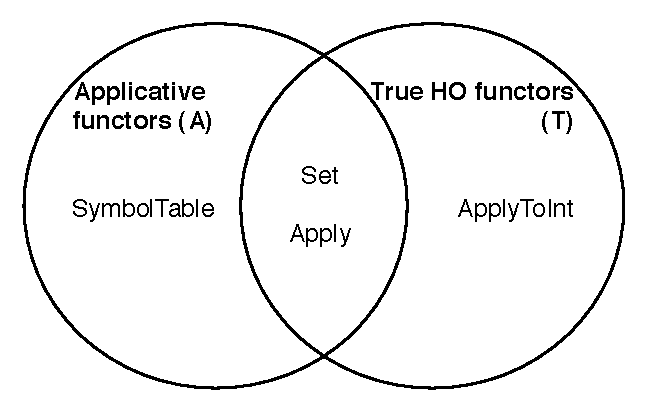
\includegraphics[scale=0.5]{design/figs/appandtruetypeprogvenn.pdf}
% \caption{The sets of programs that type propagates through HO functor application under applicative and true HO functor semantics overlap but are not subsets of each other. Non-fully transparent generative functors do not propagate types for any of these programs.}
% \label{fig:appandtruetypeprogvenn}
% \end{figure}

% Show example. explanation of related work should be self-contained "mini-essays"
In instances such as the SymbolTable functor (fig.~\ref{fig:symtbl}), applicative functors admit too much sharing as noted by Dreyer \cite{dreyerthesis}. Applicative functors would permit the symbols from one SymbolTable ST1 to be used to index another ST2 despite the sealing of the functor body to signature SYMBOL\_TABLE. Both OCaml and SML/NJ elaborators will make the symbol type abstract, but it is only abstract with respect to external clients and not other instances of SymbolTable. Because SymbolTable is applied to the same argument for both ST1 and ST2, the two instances also share the same symbol type according to applicative functor semantics. This behavior breaks an important abstraction. Generative functors are more appropriate for enforcing the exact kind of abstraction desired. In contrast, applicative functor semantics are appropriate for some purposes such as the Set functor in fig.~\ref{fig:setfct} where the type sharing of Item.item is desirable and it is acceptable to use items in Sets of the same type interchangeably. However, it is debatable whether the Set functor is a common case. I will argue that the set of programs for which true higher-order functors propagate types is exactly those one would want to propagate types. In contrast, one should not propagate types in the set Applicative functors - True HO functors. Dreyer \cite{dreyerthesis} noted correctly that applicative functors and non-fully transparent generative functors are incomparable. Neither applicative nor true higher-order functors can subsume the other. However, there remains the question whether the programs that propagate types under applicative functors but not under true higher-order functors ought to have propagated the types in those cases. 

\begin{figure}
\begin{lstlisting}
signature SYMBOL_TABLE = 
sig 
	type symbol 
	val string2symbol : string -> symbol 
	val symbol2string : symbol -> string 
	... 
end 
functor SymbolTable () = 
struct 
	type symbol = int 
	val table : HashTable.t = 
		(* allocate internal hash table *) 
		HashTable.create (initial size, NONE) 
	fun string2symbol x = 
		(* lookup (or insert) x *) ... 
	fun symbol2string n = 
	(case HashTable.lookup (table, n) of 
		  SOME x => x 
		| NONE => raise (Fail "bad symbol")) 
	... 
end :> SYMBOL_TABLE 
structure ST1 = SymbolTable() 
structure ST2 = SymbolTable() 
\end{lstlisting}
\caption{SymbolTable functor example from Dreyer\cite{dreyerthesis}}
\label{fig:symtbl}	
\end{figure}

\begin{figure}
\begin{lstlisting}
signature COMPARABLE = 
sig 
	type item 
	val compare : item * item -> order 
end 
functor Set (Item : COMPARABLE) = 
struct 
	type set = Item.item list 
	val emptyset : set = [] 
	fun insert (x : Item.item, S : set) : set = x::S 
	fun member (x : Item.item, S : set) : bool = 
		... Item.compare(x,y) ... 
	... 
end 
\end{lstlisting}	
\caption{Set functor example from Dreyer\cite{dreyerthesis}}
\label{fig:setfct}
\end{figure}

The original criticisms of the MacQueen-Tofte semantics are the lack of support for true separate compilation and that the stamp-based operational semantics makes it difficult to extend the module system and to reason about it. Many recent treatments of ML module systems abandons true higher-order functors completely due to these issues. The claim is that the type-theoretic presentations of the module system with applicative functors address these problems. This dissertation will consider the question whether an operational semantics account must necessarily be more complicated and if so, why. In contrast to recent work, this dissertation will take true higher-order module behavior and my revised elaboration-based semantics (figs.~\ref{fig:pureml},~\ref{fig:semanticobjs}, and~\ref{fig:entsems}) as the starting point for developing a formal semantics while addressing these criticisms and concerns. My formalism follows the implicit semantics in SML/NJ compiler which enriches the internal representation of functors and functor signatures to express the static actions of the functor, thus not having to do a full re-elaboration of the functor body. This approach will also yield some practical benefits. The SML/NJ and MLton implementations have not kept up with the pace of the progress in module system design at least partially due to the fact that most of the research has been a radical departure from true higher-order module semantics. Reframing the state-of-the-art in terms of true higher-order module semantics will bring recent developments closer a practical extension in these production-quality compilers. 

\subsection{Full transparency and true separate compilation}
		The main issue I will study in this dissertation is the the exact nature of the tension between true higher-order modules and separate compilation. Since MacQueen and Tofte introduced true higher-order modules, many researchers \cite{leroy94,russothesis,mixml} have studied how to downgrade higher-order functors to regain true separate compilation, by which I mean Modula-2-style separate compilation. Although Standard ML enjoys separate typechecking and compilation for the most part, the MacQueen-Tofte re-elaboration semantics of true higher-order functors necessitates the availability of the functor body source at the point of functor application. To workaround this limitation, SML/NJ uses cut-off incremental recompilation \cite{am:pldi94,hlpr:tr94} via a powerful compilation manager CM \cite{blume95:cm}. Incremental recompilation, however, does not solve the true separate compilation problem. 
		
		The separate compilation problem can be reframed as a completeness problem for the signature language, \ie, can the source-level signature language adequately describe all possible modules including functors. Currently, the SML/NJ compiler elaborates module syntax into internal semantic objects. These semantic objects are expressive enough to encode the functor body relationships that eluded the source signature language. The source and these semantic objects are then compiled to a predicative System F$_\omega$-like calculus \cite{shao98}. This suggests that an F$_\omega$-like calculus should be expressive enough to characterize all the static semantic actions of functors. 
		
		Intuitively, true higher-order modules cannot be fully expressed in the syntactic signature language because it is limited to definitional specs and type sharing. For example, there is no way to express a functor signature for the apply functor that accounts for all sharing due to full transparency. Therefore true higher-order modules cannot in general be separately compiled. In particular, HO functor applications cannot always be separately compiled from the functor definition. In the past, various researchers have approached this problem by incorporating applicative functors into the language to varying degrees \cite{leroy95,biswas95,russothesis,dhc03} sometimes limiting the generative functors in the process. In this dissertation, I will argue that applicative functors cannot replace true higher-order functors in the general case. Moreover, if fully transparent generativity is the goal, then applicative functors only serve to support true separate compilation in a limited number of cases. 
		
		% In order to have true separate compilation, the surface signature language must be able to express the full signature of all structures and functors. Even in a module language that only supports first-order functors, this requirement proves to be a problem because the signature language is be unable to express generative types in the body of a functor. Generative types in the body of a functor do not have externally expressible names prior to functor application. 
		
		Aside from describing the static semantic actions of HO functors, a signature language supporting separate compilation needs a mechanism to ensure coherence of the abstract types in imported modules. ML presently solves the coherence problem through a combination of type sharing constraints, definitional type specs, and where type clauses. In simpler module systems, the problem of coherence is not as pronounced because compilation units only import external units using definite references\cite{swasey06}. The current implementation for type sharing constraints resolution, called {\bf instantiation}, is a complicated process with a considerable amount of folklore. Simply put, instantiation constructs the free instantiation of a functor formal parameter that imposes the required amount of type sharing but no more. The instantiation phase in SML/NJ imposes a semantics stricter than that of the Definition. Instantiation guarantees inhabitability of signatures where the Definition does not. Although Harper and Pierce \cite{ATTAPL} claim that type sharing constraints can be superseded by definitional type specs in all cases, my study has identified examples (fig.~\ref{fig:crisscross}) where this is not the case absent a mechanism for signature self-reference, {\it e.g.}, \lstinline{structure M : S0 where type t = self.N.u}.

\begin{figure}		
\begin{lstlisting}
signature S0 = sig datatype s = A type t end
signature S1 = sig datatype u = B type v end

signature S3 =
sig
   structure M : S0 
   structure N : S1
   sharing type M.t = N.u and N.v = M.s
end 
\end{lstlisting}
\caption{Criss-crossing type sharing constraints cannot be reduced to definitional type specifications or uses of where type.}
\label{fig:crisscross}
\end{figure}

		Both Russo \cite{russothesis} and Swasey \etal~\cite{swasey06} have suggested that the separate compilation problem can be solved by identifying an alternate form of compilation unit, one that is not a module. OCaml, in fact, already implements such a regime. However, in the presence of true higher-order functors, these approaches merely punt on the real problem by compelling the programmer to put otherwise independent modules together in a single compilation unit and then abstracting over that unit. This dissertation will either prove definitely that true higher-order functors and true separate compilation are incompatible or develop a module system integrating these two features. 
		
\subsection{Signature calculus}
	Since the study of the true separate compilation problem points in the direction of the signature calculus, it will be fruitful to take this opportunity to reconsider the design of ML's signature language. After Harper-Lillibridge and Leroy, despite the continuing pace of the development of ML module systems, the signature language generally did not see much attention except for Ramsey \etal's paper\cite{ramsey05}. Ramsey \etal~\cite{ramsey05} describe a signature language that includes operations for post hoc manipulation such as adding, removing, rebinding components, and merging signatures. SML/NJ's semantics for \lstinline{include} is richer than the simple syntactic inclusion found in the Definition\cite{mthm97}. In particular, certain kinds of compatible signatures can be merged. In the SML/NJ 110.68 compiler, two signatures are {\bf compatible} when their overlapping specifications (\ie, specifications with the same name) have the same arity and follow the rules summarized in table~\ref{tbl:njsigmerge}. However, the current compatibility rules are inconsistent and incomplete. For example, merging an eqtype and a type specification results in an eqtype in one direction and a type in the other as shown in fig.~\ref{fig:compatmerge}. 

\begin{figure}
\begin{lstlisting}
signature S0 = sig eqtype t end
signature S1 = sig type t end
signature S2 = sig include S0 include S2 end 

S2 : sig eqtype t end

signature S0 = sig type t end
signature S1 = sig eqtype t end
signature S2 = sig include S0 include S2 end

S2 : sig type t end	
\end{lstlisting}
\caption{Unsound behavior of SML/NJ signature merging by \lstinline{include}}
\label{fig:compatmerge}
\end{figure}
	
Despite its present incomplete state, SML/NJ can do the appropriate consistent merge for Garcia \etal's example (fig.~\ref{fig:garciasigmerge}). In the case of Garcia \etal's example, the typechecker needed to do is to note that the repeated components $t$ and $u$ due to inclusion are identical specifications. 
	
	The SML/NJ semantics goes further and merges consistent yet unequal specifications such as abstract types and datatypes. The merging semantics can be substantially improved by making the table more symmetrical and adjusting some of the precedences to something more sensible. Both Ramsey \cite{ramsey05} and Dreyer and Rossberg \cite{mixml} offer language support for a signature calculus that can safely compose signatures, effectively permitting a kind of multiple signature inheritance. Both accounts only model signature merging for a small language without support to features such as eqtype and generative datatypes. In particular, a fine-grain merging of eqtype can be nontrivial. For example, it is safe to merge \lstinline{eqtype t} and \lstinline{datatype t = K} where K is a data constructor. In contrast, merging \lstinline{eqtype t} and \lstinline{datatype t = K of int -> int} is unsafe. Consistent merge rules of this flavor can already be found elsewhere in the compiler, namely in signature matching. This dissertation will develop a formal semantics for a safe but flexible consistent signature merging that covers these features of ML. 

				\begin{table}
				\begin{tabular}{|l|l|l|l|l|}
				\hline
				     & type & eqtype & datatype & deftype\\
				\hline 
				type & \chk & eqtype & \ex & \ex\\
				\hline
				eqtype & type & \chk & \ex & \ex\\
				\hline
				datatype & \chk & datatype & \ex & \ex\\
				\hline
				deftype & \ex & \ex & \ex & \ex\\
				\hline
				datatype withtype & \chk & datatype withtype & \ex & \ex\\	
				\hline
				\end{tabular} 
				\caption{SML/NJ 110.68 Signature elaboration consistent signature merging: \chk~can be merged, \ex~cannot be merged, otherwise indicates specs mergable but indicated spec takes precedence}
				\label{tbl:njsigmerge}
				\end{table}
				
\begin{figure}[ht]
\hrulefill\\
\begin{minipage}[b]{0.5\linewidth}
\begin{lstlisting}[frame=none]
signature S0 = 
  sig 
    type t
    eqtype u
  end
\end{lstlisting}
\end{minipage}
\hspace{0.1em}
\begin{minipage}[b]{0.5\linewidth}
\begin{lstlisting}[frame=none]
signature S1 = 
  sig 
    include S0
    val x : int
  end
\end{lstlisting}
\end{minipage}\\
\begin{minipage}[b]{0.5\linewidth}
\begin{lstlisting}[frame=none]
signature S2 = 
  sig 
    include S0 
    val y : unit 
  end
\end{lstlisting}
\end{minipage}
\hspace{0.1em}
\begin{minipage}[b]{0.5\linewidth}
\begin{lstlisting}[frame=none]
signature S3 = 
  sig 
    include S1 
    include S2 
  end
\end{lstlisting}
\end{minipage}
\hrulefill
\caption{The naive macro expansion semantics of the Definition rejects S3. SML/NJ accepts it. This example was derived from Garcia \etal's GraphSig, IncidenceGraphSig, and VertexListGraphSig\cite{garcia05:extendedcomparing05}.}
\label{fig:garciasigmerge}
\end{figure}

The signature merging semantics found in Ramsey \etal~is quite aggressive. In one example (fig.~\ref{fig:ramseymerge}), the merging semantics creates a new definitional type spec \lstinline{type u = t} in order to merge two signatures that disagree on an entangled value specification \lstinline{val x : t list} and \lstinline{val x : u list}. This kind of aggressiveness likely goes beyond the intention or expectation of the programmer. The programmer may have difficulty deciphering typechecking errors relating to S2.u and S2.x after this point because of this aggressive induced type sharing. It would be more sensible to have the typechecker complain that S0.x and S1.x are incompatible value specifications because as far as the typechecker and programmer are concerned, S0.t and S1.u are simply flexible type specifications. 

\begin{figure}[ht]
\hrulefill\\
\begin{minipage}[b]{0.5\linewidth}
\begin{lstlisting}[frame=none]
signature S0 =
sig
  type t
  type u 
  val x : t list
end
\end{lstlisting}
\end{minipage}
\hspace{0.1cm}
\begin{minipage}[b]{0.5\linewidth}
\begin{lstlisting}[frame=none]
signature S1 = 
sig
  type t
  type u 
  val x : u list
end	
\end{lstlisting}	
\end{minipage}\\
\begin{lstlisting}[frame=none]
signature S2 =
sig
  type t 
  type u = t
  val x : t list
end	
\end{lstlisting}
\hrulefill
\caption{This is an example from Ramsey \etal \cite{ramsey05}. S2 is the merge (greatest lower bound) of S0 and S1 according to their semantics.}
\label{fig:ramseymerge}
\end{figure}

Inspired by Ramsey \etal, my study of signature calculi will go beyond the semantics of consistent signature merging to consider the design implications of adding parameterized signatures\cite{jones96}, signature variables, and related features to the ML signature language.
The ML signature language permits type definitions that may refer to general type expressions. Type expressions may involve both primitive type constructors such as $\rightarrow$ and programmer-defined type operators. It is the inclusion of type operators that gives the signature language much of its expressiveness. The semantics of type sharing constraints differs significantly between SML90 and SML97. Type sharing constraints could be imposed on two type constructors without restriction in SML90. In SML97, the designers partitioned the semantics of type sharing into type definitions which expressed sharing between an abstract type and an arbitrary type expression, and regular type sharing constraints which can only be imposed between two flexible (or primary) types whose names must be in scope. 

				A module system that permits both type definitions and type sharing constraints in signatures introduces significant new complexity. For example, whereas in Leroy's \cite{Leroy:generativity} TypModl language, which only permits SML90-style definitional type sharing constraints and no type definitions, type sharing constraints can be ``normalized'' by pushing them up the signature and eliminated by turning them into type definitions, type sharing constraints cannot be eliminated in a language that permits both type definitions and type sharing constraints. 

In ML modules, structures can be arranged in a hierarchy. This feature enables flexible namespace management. In contrast, signatures cannot be arranged in such a hierarchy. Signatures must be defined at the top-level and can never be enclosed in any other signature or module. For complex hierarchies such the SML/NJ's Control module that contains layers of submodules, the corresponding signature CONTROL and the signatures of the submodules PRINT and ELAB are related only incidentally by occurrence in structure specifications in CONTROL. This shortcoming in the signature language unnecessarily pollutes the signature namespace and complicates browsing through and working with highly nested hierarchies. It would be desirable to permit (transparent) signature specifications within signatures. For added flexibility and perhaps increased expressiveness, it may be useful permit signature definitions within structures and functors. Furthermore, in order for modules to match these signatures enriched with signature specifications, modules must permit corresponding signature definitions. 

\begin{figure}
\begin{lstlisting}
structure M = 
  struct 
    type t = int 
    type u = bool * string 
    val a : u * t
  end 
signature S = sign(M) removing u adding val b : t * t	
\end{lstlisting}	
\caption{Accessing and modifying (via Ramsey \etal~signature operations) an inferred signature}
\label{fig:inferred}
\end{figure}

Since the semantics of ML already supports the extraction or inference of module signatures from the implementation, perhaps it makes sense to permit the programmer to operate directly on the inferred signatures of implementations (modules) or generate/synchronize module implementation based on the signature. Programmers often skip the step of writing proper signatures for modules because the necessary notation is cumbersome and potentially repetitive with respect to the module implementations of signatures. Some programming environments can help programmers automatically generate interfaces, but changes usually are not propagated bidirectionally. Synchronization of modules and signatures is ill-defined in the ML module system which supports a many-to-many relationship between modules and signatures. However, this is exactly where the existence of a principal signature or of a full signature might be useful. If programmers can leverage the structure of existing module structure when writing signatures, this might lower the barrier of entry for programmers with existing non-modularized source thus providing a path to ``gradual modularization''. For example, in fig.~\ref{fig:inferred} an inferred signature can be modified after the fact to serve as a template for future structures without having to explicitly write out any signature. This signature language will enable programmers to quickly integrate modular and non-modular code by facilitating rapid construction of variations on inferred signatures. Admittedly, this feature may run against the very spirit of splitting out explicit interfaces from implementations. 

% \section{Secondary Research Problems}
% \subsection{Static effects} including generative v. MixML mutation of types 
% \subsection{Module linking} functional and ad hoc linkage to show MixML is a radical departure from ML computational linking (the computation that happens before linking to produce the environments/closures that go along with the functions to be linked)

%% \section{Principal Goals of Research} Maybe here???
% \subsection{Polymorphism}
% \subsection{Generativity and abstraction}

\section{Related work}
Module systems have generally followed either in the extralinguistic style of Modula and Mesa or the functional style of ML. Dreyer and Rossberg's recent module system leans towards the extralinguistic style with the subtle mixin merge linking construct that serves many roles including encoding functor application. Cardelli \cite{cardelli97} brought some amount of formalization to this {\it ad hoc} approach to modularity, but module systems in this style still vary considerably in terms of semantics. Moreover, the extralinguistic semantics of linking are typically fairly involved and delicate.

The ML module system has inspired a bevy of formalisms describing its semantics and common extensions. These formalisms run the gamut from Leroy's presentation based on syntactic mechanisms alone, to Harper-Lillibridge \cite{lillibridge94} and Dreyer, Crary, and Harper's \cite{dhc03} type-theoretic approach, to the elaboration semantics approach as represented by the Definition\cite{mthm97}. As I have discussed at length in sec.~\ref{sec:hofct}, full transparency is a desirable property for module system designs. Designs range from no support for transparency (type propagation) such as non-propagating functors and complete support for MacQueen-Tofte full transparency. In between are the various gradations,\ie, different combinations of applicative and generative functors.  Another important quality of the account of module system design is the formalism used for expressing the semantics. In the early days, module system semantics were quite {\it ad hoc}, each relying on their own peculiar notation and collection of semantic objects\cite{wirth:module,cacm:mesa,tofte92}. Since then, there has been a strong move toward more standardized logical frameworks that are more amenable to encoding in a theorem proving system such as Isabelle/HOL and Coq\cite{lillibridge94,dhc03}. Curiously, the most recent accounts have been moving back towards a semantic objects-based approach\cite{dreyer07,mixml}. Fig.~\ref{fig:spectrum} shows very roughly where the major families of module system designs fall in relationship to each other in terms of support for full transparency and adherence to some formal logic framework. In the figure, it appears that the left-hand side has been well-explored. I will study the right-hand side, and perhaps the upper-right-hand quadrant which represents a fully transparent semantics in something close to a mechanized metatheory for Coq. This study will ideally result in a module system design that reconciles a current understanding of fully transparent functors with a simpler and more accessible semantics, a clear evolutionary step from the state-of-the-art. 

\begin{figure}
\hrulefill
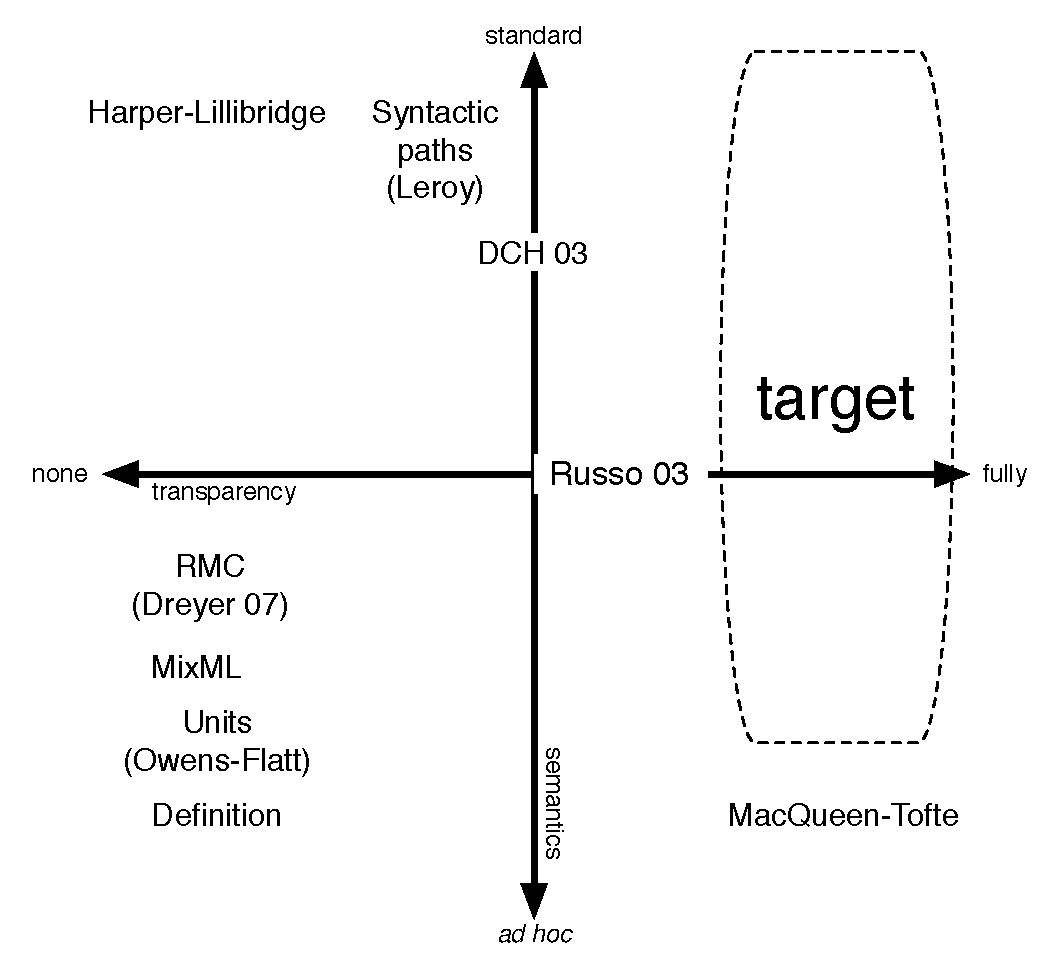
\includegraphics[scale=0.5]{../../design/figs/modsys-spectrum.pdf}
\hrulefill\\
{\small A semantics is more standard in the sense that it uses more formal logic frameworks. It may potentially be easier to mechanize the metatheory of such semantics.}
\caption{The spectrum of major module system families}
\label{fig:spectrum}
\end{figure}

Besides the main module system features described earlier in this proposal, there are a number of other useful properties developed in the different module languages. The {\bf phase distinction} \cite{hmm:phasedist} plays a fundamental role in ensuring that module systems can be typechecked fully at compile-time. This property is desirable, being consistent with our goal of static type safety. It says that a language, in this case a module, can be split into static and dynamic parts such that the static part does not depend on the dynamic. Some accounts of module systems respect phase distinction at the surface language level \cite{leroy95,russothesis}. Others respect the phase distinction in an internal language but not the surface language \cite{mt94}.  

The other key property in a module system design is the existence of a {\bf principal signature} for modules. The term principal signature has been overloaded in meaning. Because of the many-to-many relationship between signatures and modules and the signature subtyping relationship, many signatures may be safely ascribed to a single structure. I will call the most precise signature for a structure (i.e., one that constrains all components of the structure with exact, most constraining types) the {\bf full signature}. A related concept is the {\bf free instantiation} of a functor formal parameter. The free instantiation is an instance of the functor formal parameter signature S that admits exactly enough type sharing to satisfy $S$ and no more. In particular, it avoids any extraneous type sharing that would constrain the free instantiation more than is necessary. What Dreyer\cite{dreyerthesis} calls the principal signature is the full signature in this terminology. Tofte defines principal signature of a signature expression $sigexp$ as one whose flexible components (\ie, abstract types) can be instantiated to obtain all instantiations of $sigexp$ \cite{tofte92,mthm97}. I will adopt Tofte's terminology. 
 
\subsection{Type-theoretic approach}
Beginning with Harper-Lillibridge's translucent sums module calculus \cite{lillibridge94}, this large, prolific family of module systems pushed the state-of-the-art in terms of the type theoretic approach to module system design. Although Harper-Lillibridge originally explored first-class modules, the bulk of the research in this family was directed towards an applicative higher-order module semantics for type-directed compilers TIL/TILT and adding recursion. 

Crary \etal~\cite{crary99} and later Dreyer \cite{dreyer04,dreyer07} have explored adding support for recursion. Harper-Lillibridge \cite{lillibridge94} and then Russo \cite{russo00} studied mechanisms for making modules first-class entities in the core language. With first-class modules, programmers can leverage the familiar module system to take advantage of the System F-like power of the module system for programming-in-the-small. Unfortunately, as Garcia \cite{garcia05:extendedcomparing05} remarks, the syntactic overhead of the ML module system makes this undesirable and impractical. When used in a similar context, Garcia suggests that the type inference used for type classes makes modular programming-in-the-small more succinct. This observation holds only in specialized use case of type classes. 

\subsection{Syntactic paths approach}
One of the first formal accounts of an ML-like module system is Leroy's manifest types calculus\cite{leroy94} where manifest types are definitional type specifications. The surface language for the manifest types calculus is equivalent to that of the translucent sums calculus described by Harper-Lillibridge. The key observation in the manifest types calculus is that one can typecheck manifest types by comparing the rooted syntactic paths to those types which uniquely determine type identity. Thus, type equivalence is syntactic path equivalence. Leroy introduced the notion of applicative functors which held types in the result of a functor application to be equivalent to corresponding types in all other results of applications of that functor to the ``same'' argument\cite{leroy95}. There is a design space for module equivalence, from static equivalence to full observational equivalence. Several designs \cite{shao99,dhc03,russothesis} have tried to incorporate both applicative and generative functors in a single calculus. Cregut \cite{CregutMacQueen94} enriched signatures with structure equalities to obtain complete syntactic signatures for separate compilation.

Leroy introduces a relatively simple approach to module system semantics that precludes shadowing of core and module bindings \cite{Leroy:generativity,leroy00}.
The semantics supports type generativity and SML90-style definitional sharing by reducing them to solving path equivalence by way of A-normalization (for functor applications) and S-normalization (a consolidation of sharing constraints by reordering). In his module system, Leroy claims that all type sharing can be rewritten in his calculus with generative datatypes and manifest types. However, Leroy's simplified module system does not include value specifications and datatype constructors both of which can constrain the order in which specifications must be written and therefore result in situations where sharing constraints cannot be in general reduced to manifest types. 

For full transparency, Leroy proved that there is a type-preserving encoding of a stratified calculus with strong sums without generativity using applicative functors\cite{leroy95}, claiming that the existence of such an encoding is a strong hint that applicative functors support full transparency. My HO apply functor example in fig.~\ref{fig:hoapplyfct} casts some doubt to this claim. As Leroy pointed out, under the strong sums model, first-class modules is at odds with phase distinction because of the typechecker would have to do arbitrary reductions\cite{leroy94}. In contrast, because the weak sum model of the manifest types calculus does not require any reductions at typecheck time regardless of the presence of first-class modules, it does not violate the phase distinction\cite{leroy94}. In the most recent paper in the manifest types series \cite{leroy00}, Leroy abstracts away most of the core language details from the manifest calculus to obtain a mostly core language independent module system. 

Shao \cite{shao99} offers a signature language based on gathering (and internally factoring out) all flexible components (\ie, abstract type components unconstrained by sharing) in a higher-order type constructor that can be applied to obtain a signature that expresses functor body semantic actions at a later point. The resultant signature language superficially resembles applicative functors. However, type constructor applications in the signature language must be on paths. Consequently, it does not support full transparency in the general case. 

Although the syntactic paths approach may very well provide the simplest account of module systems, this is at the cost of some very fundamental shortcomings such as the inability to support shadowing and full transparency. Because the account's support for type sharing is incomplete, there may also be limits to how the semantics deals with the coherency issue. The proposed dissertation will address these issues which are fundamental to the power of the ML module system. 

\subsection{Moscow ML}
Biswas gave a static semantics for a simpler form of higher-order modules\cite{biswas95}. The account relies on semantic objects and a stamp-based semantics similar to the Definition. The type propagation in higher-order functors is captured by a ``higher-order'' dependency variable that abstracted possible dependencies on the argument. These variables are only present in the internal language produced during elaboration. Consequently, Biswas's semantics does not support true separate compilation and neither does it enrich the surface syntax for signatures. Biswas's elaboration rule in fig.~\ref{fig:biswas-abstypespec-elab} maps an abstract type name t to the fresh higher-order abstract dependency variable $f$ applied to the list of all abstract dependency variables $\mathcal{W}$ it could possibly depend upon. For example, the functor parameter of the Apply functor, \lstinline{functor F(X:sig type t end): sig type t end}, is given the semantic representation $\forall f_0(\{t\mapsto f_0\} \Rightarrow \{t\mapsto f_1(f_0)\})$.

\begin{figure}
\AxiomC{$f$ is a fresh higher-order dependency variable}
\UnaryInfC{$\Gamma,\mathcal{W}\vdash\mathrm{type~t}\Rightarrow ((t \mapsto f(\mathcal{W}), \emptyset), \{f\})$}
\DisplayProof\\
\caption{Biswas's elaboration rule for abstract type specifications: $\Gamma$ is the type environment mapping program variables to types. $\mathcal{W}$ is a list of formal parameters variables the specification may depend on.}
\label{fig:biswas-abstypespec-elab}
\end{figure}


Biswas's formal account was extended in a somewhat more type-theoretic style to the full SML language and implemented by Russo in the Moscow ML compiler. Moscow ML also adds support for first-class modules\cite{russo00} and a form of recursion\cite{russo01}. This family of semantics attempts to incorporate both non-propagating generative functors and applicative functors. The main limitation, as pointed out of Dreyer \cite{dreyerthesis}, is that Moscow ML's combination of generative and applicative functors is unsound. In particular, any generative functor can be $\eta$-expanded into an applicative functor thereby circumventing the generative functor abstraction. 

\subsection{Units and other extralinguistic linking system}
Flatt-Felleisen \cite{ff98} and Owens-Flatt \cite{owensflatt06} develop a module system semantics based on a calculus with stratified distinct hierarchically composable modules and recursively linkable units. Because both accounts appeal to extralinguistic linking semantics, they fall under the Module/Mesa line of module systems. As pointed out of Dreyer\cite{mixml}, the fundamental limitation in this semantics is that the stratification of units and modules makes precludes using unit linking and hierarchical composition together. One strength of their module system design is that it is one of the few accounts that includes an operational dynamic semantics, unlike all the other accounts discussed in this section. All other accounts of module systems merely give a static semantics and perhaps a typechecking algorithm which they prove is sound with respect to the static semantics. Owens and Flatt prove type soundness of their semantics. 

Swasey \etal~\cite{swasey06} described a calculus SMLSC that is modeled after Cardelli's linkset approach to separate compilation. SMLSC introduces a compilation unit that sits on top of the module system that can be separately compiled from unimplemented dependencies by means of a handoff units whose role resembles that of header files in C.

\subsection{The Definition and MacQueen-Tofte}
The Definition of Standard ML \cite{mth90,mthm97} semantics for the module system evolved throughout the late 1980s and early 1990s. Early on, Harper \etal~gave a fairly complete account of the static semantics of the first-order ML module system in terms of an operational stamp-based semantics\cite{hmt:tapsoft87}. Tofte proves that signature expressions in the first-order, generative semantics have principal signatures in his thesis \cite{toftethesis}. He also extended this proof to cover non-propagating higher-order generative functors\cite{tofte:jfp94}. Then MacQueen and Tofte introduced true higher-order functor semantics\cite{mt94}. 

%Key to the semantics is the partitioning of structures into signature and {\bf realization} halves. A signature is the skeletal form of the structure, \ie, type and value specifications, with flexible type specifications that can be instantiated by signature matching. A realization fills in these flexible type specifications. 

Apart from type propagation transparency issues, the evolution of the Definition also addressed other key issues type sharing issues. The role of {\bf type sharing constraints} has evolved through the development of the Standard ML semantics and SML/NJ implementation. Type sharing constraints solve two problems in ML, type specification refinement and coherence. Originally, type specifications only declared the name of an expected type. It is quite useful to be able to refine type specifications to restrict it to particular definite types. The coherence problem is the challenge of constraining type components of two structures which may or may not be identical to be equivalent regardless of the actual identity of that type. In SML90 \cite{mth90}, explicit sharing equations among visible abstract types and generative structure sharing served as the sole means for constraining type specifications. Under generative structure sharing semantics, each structure had a unique identity. Thus, two structures shared only when they were identical in the sense that they were defined at the same point in the program and are merely aliases (fig.~\ref{fig:structuresharing}). Structures that shared in this sense were equivalent both statically and dynamically. This kind of rich sharing semantics turned out to be quite complicated and was soon abandoned in favor of a structure sharing that simply reduced to type sharing constraints on the type specifications inside the signature. 

\begin{figure}
\begin{lstlisting}
signature S0 = 
sig 
  type t
  val f : t -> t
  val state : t ref
end

functor F(X:sig 
              structure A : S0
              structure B : S0
              sharing A = B
            end) = ...

functor G() = 
struct
  type t = unit
  val f = ...
  val state = ref 0
end

structure M0 = G()
structure M1 = G()
structure M2 = M0

structure M3 = F(struct 
                   structure A=M0
                   structure B=M2
                 end)

structure M4 = F(struct
                   structure A=M0
                   structure B=M1
                 end)
\end{lstlisting}
\caption{Under SML90 identity-based structure sharing, A and B have to be aliases, so the functor application at M4 fails to typecheck. Under SML97, the sharing constraint merely rewrites to sharing type A.t = B.t, thus both functor applications typecheck. }
\label{fig:structuresharing}
\end{figure}

SML93 introduced definitional type specifications, giving programmers two ways for constraining types to definite ones. SML97 added where type and definitional type specifications completely replaced the definitional type sharing found in SML90. Definitional type specifications and type sharing were finally disentangled. Generative structure sharing was eliminated in favor of the simpler semantics of a structural sharing that amounted to a type sharing equation for each common type specification, no matter how deeply nested. The semantics of type sharing and related mechanisms such as \lstinline{where type} are still somewhat problematical and unsettled\cite{narbel:jfp07,ramsey05}. Type sharing as it stands gives rise to a delicate and non-obvious resolution algorithm, {\bf instantiation}. Ramsey \etal~has argued that the scoping of \lstinline{where type} definitions should be more symmetric thereby permitting more flexible type specification refinements.

% In MacQueen-Tofte (MT), signatures support higher-order functors by including a functor signature environment, denoted $\Phi$, that maps functor maps to functor signatures. Because signatures of functor components may depend on specifications that came earlier in the enclosing structure signature, the system introduces a binding $\lambda\rho$ that binds $\rho$, the entity variable representing the entire enclosing structure signature. 
% 
% The MT structure signatures require this $\lambda\rho$ binding because they incorporate functor signature environments indexed by functor paths, $\Phi$. Without the $\lambda\rho$-binding, $\Phi$ cannot depend on entities in the enclosing signatures. Structure matching first looks up all $fp$s in $\Phi$ and then attempts to match the static functor with $\Phi[\varphi/\rho]$.

%Signature specifications contain the signatures and realizations for structure definitions 
%(\ie, $\rho,\Sigma=\Sigma$ and $\rho,\Sigma=_{\overline{\rho}} \Sigma$) 
% at the point of structure signature matching. These definition structure signatures and realizations are filled in during signature elaboration by looking up the static environment and entity path context. 

Shao \cite{shao98} (in a paper unrelated to the one on applicative functor-like module system \cite{shao99}) extends MacQueen-Tofte fully transparent modules with support for type definitions, type sharing (normalized into type definitions), and hidden module components. This treatment of higher-order modules is a more recent form of what is currently in the SML/NJ compiler. Elsman presents a module system compilation technique used in the ML Kit compiler \cite{elsman99}. The semantics follows the style of the Definition. The compilation technique is comparable to Shao's FLINT compilation scheme. 

The SML/NJ compiler implements a version of the module system that departs from the Definition in a number of aspects. Some of these extensions have not been formalized as of yet. In particular, the compiler has a richer semantics for \lstinline{include} and the elaborator now compiles a functor body to a static lambda calculus which is what is used in place of the actual functor body during the re-elaboration at application. The scoping of sharing constraints has also changed. In the current implementation, SML/NJ no longer permits nonlocal forms of sharing of the flavor illustrated in the example in MT (fig.~\ref{fig:nonlocalsharing}). Instead, structure definitions express the same kind of sharing. The module system also has some significant limitations such as recursion, the tension between separate compilation and fully transparent generative functors, and the limited signature language.

\begin{figure}
\begin{lstlisting}
structure S = struct end;
signature SIG = 
sig
  structure A : sig end
  structure B : sig end
  structure C : sig end
  sharing A = S
  sharing B = C
end	
\end{lstlisting}	
\caption{In the current implementation of SML/NJ, the first kind of sharing constraint is no longer permitted. Both sides of the constraint must be in local scope as is in the second sharing constraint.}
\label{fig:nonlocalsharing}
\end{figure}

\subsection{Alice ML}
Alice ML provides a number of the features mentioned in this proposal especially in the 
area of signature language enrichments. The language supports nested signatures of both varieties: those that must be repeated in the signature for the enveloping structure and those that are abstract. The abstract signatures do not, however, appear to be complemented with any bounded polymorphism features. 

\subsection{MixML}
		Dreyer and Rossberg \cite{mixml} show how to encode ML signatures, structures, and functors in a mixin module calculus that appeals to something similar to Bracha's merge\cite{bracha:thesis} as its only linking mechanism. When linking a module A and B, the semantics tries to satisfy the imports of A using the exports of B and vice versa. The mixin merging syntax is {\bf link} x=M0 {\bf with} M1 in the surface language. It binds the name x to a module M0 and concatenates it with M1 merging components where appropriate. The scope of x is the body of M1. This mixin merging semantics supports recursion and separate compilation. Modules in this language consist of atomic modules that only contain values, types, type constructors, {\it etc}., labeled modules ($\{\ell = M\}$), and the merging form link ... with ....  

The peculiarity in this language is that modules and indeed anything that can be encoded in these modules are stateful. For example, signatures in MixML are fundamentally stateful. Linking against a signature S mutates it. Consequently, the typechecker rejects the following program. 
\begin{lstlisting}
module U = link x={module S = {type t}} 
           with {module A=(link x=x.S with {type t = int}), 
                 module b=(link x=x.S with {type t = bool})};		
\end{lstlisting}
Signatures must be suspended and then new'ed in order to be matched multiple times. This suspension is called a unit in Dreyer and Rossberg's terminology. Functors are also represented by suspending modules with unsatisfied imports. Although units have full support for hierarchical composition, MixML's design still retains the problem of stratifying modules and units, a problem inherited from the Flatt-Felleisen units that inspired it. 

%     In a bout of weird behavior, the following is rejected although the semantics suggests that it should be accepted:
% \begin{lstlisting}
% 	module U = link x={module S={type t}} 
% 	           with {module A=(link x=x.S with {type t = int}), 
% 	                 module b=(link x=x.S with {type t=int})};
% \end{lstlisting}
% 				 	There seems to a restriction that type imports can never be mentioned more than once.
% \begin{lstlisting}
% 	module U = link X = {module S = {type t}} 
% 	 		   with {module A=X.S, module B=X.S};
% \end{lstlisting}
% 	This is a restriction even if the import is linked away using the with operator. 
% 	But this restriction doesn't apply to the module being linked.
% \begin{lstlisting}
% 	(X={S={t=[:0]}}) with {A=X.S}
% \end{lstlisting}

	% Going beyond mere translucency (mixture of transparent and opaque types), one have relatively defined types (\lstinline{type s}, \lstinline{type t = s list}).
	% 
	% C has a way to import an abstract type t by some kind of empty typedef. Semantics of binding with is odd because X refers to complete module even when the module is a signature. Binding is not really an abbreviation equality. It is more of \lstinline{(X : mod) with mod} not \lstinline{(X = mod) with mod}.

	As it stands, the part of the MixML language that encodes the ML module system is but a small fraction of the whole. The question remains what implications the rest of the language has. Part of the language is obviously semantically meaningless such as {\bf link} X = [int] {\bf with} [3], which is a well-formed program. The approach that the proposed dissertation's semantics will take is to extricate the part of MixML that encodes the ML module system and hopefully simplify the semantics by omitting the rest of features. One feature I think is worth pursuing is the fact that in MixML signatures can be composed together. In ML, one can only project on modules. MixML \cite{mixml} loosens this restriction by conflating signatures and modules. Signatures can be projected out of an enclosing signature. 
%\subsection{Moby}
% \subsection{Scala}
% Scala supports encoding some of the ML module system via its structured types feature. Because of its mainly nominal typing heritage, it remains unclear how faithful is its encoding of higher-order functors. 

% \subsection{FZip}
%   Montagu and R\'emy \cite{Montagu-Remy:popl09:fzip} recently introduced a new module calculus based on existential types for encoding generativity. 

\subsection{First-class polymorphism inference and type classes}
	Jones \cite{jonesfcp} motivated first-class polymorphism (FCP) by appealing to the constructive logic tautologies for existentials, universals, and implication \cite{jonesfcp}. I observed that the constructive logic rule $\langle w, \tau_w\rangle \rightarrow \tau' \leftrightarrow w \Rightarrow \tau_w \rightarrow \tau'$ corresponds to the FLINT transformation (currying) in the forward direction and an uncurrying operation, perhaps a kind of module inference. At any rate, I would like to investigate the use cases for FCP where modules would be sufficient. More recent first-class polymorphic calculi such MLF\cite{Lebotlan-Remy/mlf-icfp} and FPH \cite{fph} add some limited type inference. Although inference in general may be undecidable, these limited inferencers still go a long way to make programming in these first-class polymorphic calculi more practical. If some of the ideas for inference for FCP calculi can be transferred over to a module calculus, one might also address the syntactic overhead of ML module systems. Adding FCP to the core introduces a certain amount of redundancy with respect to the FCP afforded by the module system. It would be useful to consider what exactly is redundant and whether that can be minimized. 
		
	Another language construct related to module systems that enjoys type inference is the type class. Type classes are a special case of modular programming where a kind of automatic deduction would be useful. Unfortunately, the scope of class instances are global. In Modular Type Classes, Dreyer \etal~ \cite{dhck07} develop semantics and a translation from type classes to a stylized use of the ML module system. I hypothesize that the type inference features of type classes might be able to be ``back-ported'' to module systems. 

\subsection{Summary}
Not all module system designs enjoy the principal signature and phase distinction properties.  Fig.~\ref{fig:sys-features} summarizes the key features of the main ML-like module system families. Note that many module systems have various combinations of these features, but none are complete. Ideally, a module system would have true higher-order semantics and all the other features except for applicative functors which would be redundant. 

\begin{figure}
	\small
\begin{tabular}{|l|l|l|l|l|l|l|l|}
	\hline
System & higher-order & first-class & sep comp & rec & app & gen & phase\\
	\hline
	HL \cite{lillibridge94} & \ex & \chk & \chk & \ex & \ex & \ex & \chk \\
	\hline
	Leroy \cite{leroy95} & \ex & \ex & \chk & \ex & \chk & \ex & \chk \\
	\hline
	Russo \cite{russo01} & \ex & \chk & \chk & \chk & \chk & \chk & \chk \\
	\hline
	DCH \cite{dhc03} & \ex & \chk & \ex & \ex & \chk & \chk & \chk \\
	\hline
	RMC \cite{dreyer07} & \ex & \ex & \ex & \chk & \ex & \chk & \chk\\
	\hline
	%$\lambda^{\llparenthesis~\rrparenthesis}$ (\cite{ATTAPL}) & & & & & & \\
	%\hline
	%$\lambda^S$ (\cite{ATTAPL}) & & N & & N & N & N \\
	%\hline
	MT \cite{mt94} & \chk & \ex & \ex & \ex & \ex & \chk & \chk \\
	\hline
	MixML \cite{mixml} & \ex & \chk & \chk & \chk & \ex & \chk & \ex \\
	\hline
	Ideal & \chk & \chk & \chk & \chk & \ex & \chk & \chk \\
	\hline
\end{tabular}\\
higher-order = true higher-order\\
rec = recursive modules\\
app = applicative functors\\
gen = non-propagating generative functors\\
phase = respects the phase distinction
\caption{A comparison of major ML-like module systems}
\label{fig:sys-features}
\end{figure}												
				
\section{Methodology}
	Informed by MixML, MacQueen-Tofte semantics, and FLINT semantics as the main sources of inspiration, my dissertation research will define a new formal semantics (including a dynamic semantics) and type system for true higher-order module system based on the current module system design in the SML/NJ compiler. The semantics will clarify and extend the implicit compiler semantics. Part of this study will include experimental prototypes evaluated according to the design criteria outlined above. This prototype module system will validate the practicality of the formal design. The prototype will include a module language elaborator including typechecker and basic compilation into a suitable typed intermediate language. 
	
	Through the course of formalizing the module system, the dissertation will establish type soundness of the module language for the dynamic semantics and type system in the style of Owens-Flatt but for the more powerful ML module system. Moreover, it will precisely define full transparency, separate compilation, and the relationship between the two. The hypothesis is that these two features are mutually exclusive because I conjecture that typechecking a signature language powerful enough to encode all possible relationships between functor parameter and body would be undecidable. If the hypothesis turns out to be false, then the dissertation should develop a signature calculus powerful enough to represent all possible static semantic actions of higher-order functor application. The final component of the dissertation will be the decidability and soundness of the signature calculus typechecking. 

	\subsection{Primary and secondary components}
	SML/NJ's implementation of elaboration and translation into the FLINT language offers some unique insight into the semantics of the module system. These insights are not merely implementation choices or details. They reflect novel fundamental issues in the design and understanding of module systems. In studying translation, it has become clear that not all abstract type components are equal. The form of a functor argument is constrained by the functor parameter signature possibly modified by a where type definition. In the parameter signature, there can be structure specifications, formal functor specifications, structure/type sharing constraints, and two classes of type specifications. Type specifications may be abstract or definitional. Abstract type specifications that remain abstract after the elaborator resolves all sharing and where type constraints are called flexible or primary components. These primary type components are those essential components that must be kept to maintain the semantics of functor application (\ie, the type application associated with the functor application). The specific function of primary type components is to capture a canonical representative of an equivalence class of abstract types induced by type sharing constraints. Each equivalence class has exactly one primary type component that serves as a representative element. References to all other members of the equivalence class should be redirected to the associated primary type component. The remaining type components are secondary and therefore should be fully derivable from the primary components and externally defined types. Secondary types do not have to be explicitly represented in the parameter signature because all occurrences of these secondary types can be expanded out according to their definitions. 

\begin{lstlisting}
functor F(type s 
          type t 
          type u = s * t
          sharing type t = s) = ...
\end{lstlisting}

	In the above example, \verb|s| can be primary, representative for the equivalence class containing both \verb|s| and \verb|t|, and \verb|u| is secondary.  

% Elsa Gunter, Faninguin (Mike Gordon's student) tried to develop a formal metatheory of Definition ML
% Peripheral goal of formalizing in 
% \section{Applications}
% \subsection{Type functionals vs. applicative functors}
% \subsection{Implied associative types}
% \subsection{Effects}

\section{Conclusion}
		ML module systems have evolved throughout the last decade by avoiding the implications of true higher-order functors and adopting a combination of applicative and opaque generative functors. At the cost of the complexity of two coexisting kinds of functors and the loss of some abstraction power, recent module systems gained true separate compilation. This dissertation will revisit true higher-order functors, motivated by the search for the exact nature of the relationship between true higher-order functors and true separate compilation. Because the problem of true separate compilation concerns the expressiveness of the signature calculus, I will also take this opportunity to revisit the ML signature calculus and extend it to support more flexible modular software composition. 

\bibliography{../../design/modules}
{

%Would a completely nondependent module calculus work? More to the point, signature specs may depend on module terms, but is there a way to avoid this kind of dependence? 
% Put figure in appendix: Preliminary (incomplete) semantics for true higher-order modules based on compiler
\appendix
\section{Initial progress on formal semantics}
The following is a summary of an initial progress on the formalization of the true higher-order module semantics found in SML/NJ 110.60+. It is a work-in-progress. Fig.~\ref{fig:pureml} summarizes the surface module calculus. It supports higher-order functors, sharing constraints, eqtype, and exception specifications. Figs.~\ref{fig:statsem}, \ref{fig:elabsig}, and \ref{fig:elabmod} give the first few rules of the elaboration semantics. More importantly, fig.~\ref{fig:semanticobjs} gives the internal module representation including for higher-order functors and the static lambda calculus of entities. Fig.~\ref{fig:entsems} describe how entities are evaluated.

%!TEX root = ../principles.tex
\begin{figure}
\centering
\fixedCodeFrame{
\small
\[
\setlength{\tabcolsep}{0ex}
\renewcommand{\arraystretch}{1.1}
\begin{array}{rcll}
	d & ::= &\signature~s=\sig{\overline{spec}}\\
	  & ~~\bnfalt& \local~\overline{d}~\inx~\overline{d}~\en\\
	  & ~~\bnfalt&~ld\\
	ld & ::= & \structure~X~=~m\\
	   & ~~\bnfalt&\functor~F\overline{(X:sigexp)}~cnstr = m\\
	   & ~~\bnfalt&\val~x=e~\bnfalt~\type~\overline{\alpha}~t=\tau\\
	   & ~~\bnfalt&\local~\overline{ld}~\inx~\overline{ld}~\en\\
	   & ~~\bnfalt&\open~\overline{q}\\
	m & ::= & q~\bnfalt~\struct{\overline{ld}}~\bnfalt~q~arg~\bnfalt~\letx~\overline{d}~\inx~m~\en\\
	  & ~~\bnfalt~&~m:sigexp~\bnfalt~m:>sigexp\\
	arg & ::= & ( \overline{d} )~\overline{arg}~\bnfalt~(m)~arg~\bnfalt~(m)~\bnfalt~(\overline{d})\\
	cnstr & ::= & :~sigexp~\bnfalt~:>~sigexp\\
	sigexp & ::= & s~\bnfalt~\sig{\overline{spec}}~\bnfalt~sigexp~\where~\type~\overline{\alpha}~q=\tau\\
	spec & ::= & \structure~q:sigexp[=q]\\
	     & ~~\bnfalt &\functor~q~\overline{(X:sigexp)} : sigexp\\
	     & ~~\bnfalt &\type~\overline{\alpha}~t[=\tau]~\bnfalt~\val~x:\tau~\bnfalt~\sharing~\type~p=p\\
	     & ~~\bnfalt &\sharing~p=p~\bnfalt~\exception~exn\\
	     & ~~\bnfalt & \eqtype~\overline{\alpha}~t[=\tau]\\
	\tau & ::= & \tau\rightarrow\tau~\bnfalt~\Int~\bnfalt~t\\
\end{array}
\]
}
The overline notation indicates a vector of the components. 
\caption{Module surface language: Design caveat -- In SML/NJ the AST permits signature declarations within structures. The parser, however, does not support this. The surface language follows the parser. The implementation AST has an Abstract Structure form, but the parser does not seem to ever produce it. }
\label{fig:pureml}
\end{figure}
%!TEX root = ../principles.tex
\begin{figure}
\centering
\fixedCodeFrame{
\small
\[
\setlength{\tabcolsep}{0ex}
\renewcommand{\arraystretch}{1.1}
\begin{array}{ll}
	\infer[\rlabel{local}]{\begin{array}{l}\Gamma\vdash\local~\overline{d_1}~\inx~\overline{d_2}~\en\\
	\Rightarrow(\underline{\local}~\underline{\overline{d_1}}~\inx~\underline{\overline{d_2}}~\en,entdec,\Gamma_2,\Delta)\end{array}}
		{\Gamma\vdash\overline{d_1}\Rightarrow(\underline{\overline{d_1}},entdec_1,\Gamma_1,\Delta_1)\\ 
 \Gamma\oplus\Gamma_1\vdash\overline{d_2}\Rightarrow(\underline{\overline{d_2}},entdec_2,\Gamma_2,\Delta_2)}
\\
\qquad
\\
\infer[\rlabel{type}]{\Gamma\vdash\type~\overline{\alpha}~t=\tau\Rightarrow(,entdec,\Gamma,\Delta)}
{\strut}
\\
\qquad
\\
\infer[\rlabel{sig}]{\Gamma\vdash\sig{\overline{spec}}\Rightarrow(\sig{\overline{spec}},\bullet,\Gamma',\emptyset)}{\strut}
\\
\qquad
\\
\infer[\rlabel{structure}]{\Gamma\vdash\struct{\overline{ld}}\Rightarrow\struct{\overline{ld}}}{}
\end{array}
\]
}
The underline notation denotes the elaborated version of the nonterminal, i.e., the explicitly typed and elaborated variant.
\nocaptionrule
\caption{Static Semantics}
\label{fig:statsem}
\end{figure}
\input{../../design/figs/fig-rlzn}
\input{../../design/figs/fig-evalent}
%!TEX root = ../principles.tex
\begin{figure}
\centering
\fixedCodeFrame{
\small
\setlength{\tabcolsep}{0ex}
\renewcommand{\arraystretch}{1.1}
~\\[2mm]
\fbox{$\Gamma,\Upsilon,\Sigma\vdash sigexp \Rightarrow_{sig} \Sigma'$}
	
\begin{equation}
\infer{\Gamma,\Upsilon,\Sigma\vdash x \Rightarrow_{sig} \Gamma(x)}
{\strut} 
\label{eq:emptysig}
\end{equation}

\begin{equation}
\infer{\Gamma,\Upsilon,\Sigma\vdash sigexp~\textbf{where type}~p = C^\lambda\Rightarrow_{sig}\mathsf{rebind}(p,\mathbb{C}^\lambda,\Sigma')}
	{\begin{array}{c}
	  \Gamma,\Upsilon,\Sigma\vdash sigexp\Rightarrow_{sig}\Sigma'\qquad
	  \Sigma'(p) = (\rho,n)\\ \Gamma,\Upsilon\vdash C^\lambda \Rightarrow_{tyc} \mathfrak{C}^\lambda\qquad 
          \Gamma,\Upsilon,\Sigma\Sigma'\vdash C^\lambda \searrow^{tyc} \mathfrak{C}^\lambda \\
          \Upsilon\vdash \mathfrak{C}^\lambda \searrow^{tyc} 
          \mathbb{C}^\lambda\qquad |\mathbb{C}^\lambda|=n
	 \end{array}} 
\label{eq:wheretype}
\end{equation}

\begin{equation}
\infer{\Gamma,\Upsilon,\Sigma\vdash \textbf{sig } specs \textbf{ end} \Rightarrow_{sig} \Sigma'}
	{\begin{array}{c}
	\Gamma,\Upsilon,\Sigma\vdash specs \Rightarrow_{specs} \Sigma'
	\end{array}} 
\label{eq:sigspecs}
\end{equation}

$\mathsf{rebind}(p,\mathbb{C}^\lambda,\Sigma)$ replaces the
binding $[x\mapsto (\rho,n)]$ in $\Sigma$ with $[x \mapsto 
\mathbb{C}^\lambda]$ where $p$ ends in $x$. 

\fbox{$\Gamma,\Upsilon,\Sigma\vdash specs \Rightarrow_{specs} \Sigma$}
\begin{equation}
\infer{\Gamma,\Upsilon,\Sigma\vdash \emptyset_{specs} \Rightarrow_{specs} \emptyset_{sig}}
{\strut}
\end{equation}

\begin{equation}
\infer{\Gamma,\Upsilon,\Sigma\vdash spec,specs \Rightarrow_{specs} \Sigma'\Sigma''}
{\Gamma,\Upsilon,\Sigma\vdash spec \Rightarrow_{spec} \Sigma' \qquad \Gamma,\Upsilon,\Sigma\Sigma'\vdash specs \Rightarrow_{specs} \Sigma''}
\label{eq:specs}
\end{equation}

}
\caption{Signature elaboration}
\label{fig:elabsig}
\end{figure}

\begin{figure}
	\centering
	\fixedCodeFrame{
	\small
	~\\[2mm]
	\fbox{$\Gamma, \Upsilon, \Sigma \vdash spec \Rightarrow_{spec} \Sigma'$}
\begin{equation}
\infer{\Gamma,\Upsilon,\Sigma\vdash\textbf{type
                  }\vec{\alpha}~t\Rightarrow_{spec} [t\mapsto (\rho,|\vec{\alpha}|)]}
{(\rho\textrm{ fresh in }\Gamma\textrm{ and
                  }\Upsilon)} 
\end{equation}
% Do we need to extend the static environment during elaboration of
% the subsequent specs? The only reason we might need to is to support
% relativization. I think we have to. 
\begin{equation}
\infer{\Gamma,\Upsilon,\Sigma\vdash\textbf{type }t=C^\lambda\Rightarrow_{spec} [t\mapsto \mathbb{C}^\lambda]}
{\Gamma,\Upsilon\vdash C^\lambda \Rightarrow_{tyc} \mathfrak{C}^\lambda\qquad \Upsilon,\Sigma\vdash \mathfrak{C}^\lambda \searrow^{tyc}
 \mathbb{C}^\lambda}
\label{eq:typedefspec}
\end{equation}

\begin{equation}
              \infer{\Gamma,\Upsilon,\Sigma\vdash\textbf{val }x:T
                 \Rightarrow_{spec} [x\mapsto\mathbb{T}]}
{\Gamma,\Upsilon\vdash T \Rightarrow_{te} \mathfrak{T}\qquad \Upsilon,\Sigma\vdash \mathfrak{T} \searrow^{tyc} \mathbb{T}}
\label{eq:valspec}
\end{equation}

\begin{equation}
\infer{\begin{array}{c}
    \Gamma,\Upsilon,\Sigma\vdash\textbf{structure }x :
                  sigexp
                  \Rightarrow_{spec} [x\mapsto
                  (\rho,\Sigma')]
\end{array}}
		{\begin{array}{c}
                    \Gamma,\Upsilon,\Sigma\vdash sigexp
                    \Rightarrow_{sig}
                    \Sigma'\qquad
                    (\rho~\textrm{fresh in }\Gamma\textrm{ and
                    }\Upsilon) 
              \end{array}}
\end{equation}

\begin{equation}
\infer{\begin{array}{c}
\Gamma,\Upsilon,\Sigma\vdash\textbf{functor }f(X: sigexp_1):sigexp_2\\
   \Rightarrow_{spec} [f\mapsto(\rho,\Pi\rho_x:\Sigma_1.\Sigma_2)]
\end{array}}
		{\begin{array}{c}
\Gamma,\Upsilon,\Sigma\vdash sigexp_1 \Rightarrow_{sig}
\Sigma_1 \qquad
(\rho_x\textrm{ and }\rho~\textrm{fresh in }\Gamma\textrm{ and }\Upsilon )\\
\Gamma,\Upsilon,\Sigma[X\mapsto(\rho_x,\Sigma_1)]\vdash
sigexp_2 \Rightarrow_{sig} \Sigma_2\\
% \qquad \psi=\langle\lambda\rho_x.\Sigma_2 ;
%  \Upsilon\rangle % [4/8/10] Is this the correct closure environment? Can \Sigma_2 mention local entities? Yes, but those are local, therefore, they should be interpreted locally and not by the closure, which only interpret nonlocal entities.  
\end{array}}
\label{eq:fctspec}
\end{equation}

	}
	\caption{Signature spec elaboration}
	\label{fig:elabspec}
\end{figure}
%!TEX root = ../principles.tex
\begin{figure}
\centering
\fixedCodeFrame{
\small
\setlength{\tabcolsep}{0ex}
\renewcommand{\arraystretch}{1.1}
~\\[2mm]
\fbox{$\Gamma,\Upsilon\vdash d^m \Rightarrow_{decl} (\eta, \Gamma', \Upsilon')$}

	\begin{equation} 
          \infer{\Gamma,\Upsilon\vdash \circ
            \Rightarrow_{decl} (\bullet, \emptyset_{se},
            \emptyset_{ee})}{\strut}  
          \label{eq:emptydecl}
        \end{equation}

        \begin{equation}
          \infer{\Gamma,\Upsilon\vdash \mathbf{val}~x=e,d^m
            \Rightarrow_{decl} (\eta, [x\mapsto\mathfrak{T}]\Gamma', \Upsilon')}
          {\Gamma \vdash e \Rightarrow_{core} \mathfrak{T} \qquad
            \Gamma[x\mapsto\mathfrak{T}], \Upsilon \vdash d^m \Rightarrow_{decl}
            (\eta, \Gamma', \Upsilon')}
          \label{eq:valdecl}
        \end{equation}

	\begin{equation} 
          \infer{\begin{array}{l} 
              \Gamma,\Upsilon\vdash \mathbf{type}~t=C^\lambda,d^m
              \Rightarrow_{decl}(\eta,[t\mapsto \mathfrak{C}^\lambda]\Gamma',\Upsilon')
	\end{array}}
	{\begin{array}{c}
            \Gamma,\Upsilon \vdash C^\lambda \Rightarrow_{tyc} \mathfrak{C}^\lambda\qquad
            \Gamma[t\mapsto \mathfrak{C}^\lambda],\Upsilon\vdash
            d^m\Rightarrow_{decl}(\eta,\Gamma',
            \Upsilon')
          \end{array}} 
        \label{eq:typedefdecl}
      \end{equation}

        \begin{equation} 
       \infer{\begin{array}{c}
           \Gamma,\Upsilon\vdash
         \mathbf{datatype}~\vec{\alpha}~t,d^m\\
         \Rightarrow_{decl}([\rho_t =_{tyc} \newx(n)]\eta, [t\mapsto
         \tau^n]\Gamma', [\rho_t\mapsto \tau^n]\Upsilon')
       \end{array}}
{\begin{array}{c}
    n=|\vec{\alpha}|\qquad
    \Gamma[t\mapsto\tau^n],\Upsilon[\rho_t\mapsto \tau^n]\vdash d^m \Rightarrow_{decl} (\eta, \Gamma',
    \Upsilon')\\ (\rho_t\textrm{ and }\tau\textrm{ are fresh})
\end{array}}
      \label{eq:dtdecl}
        \end{equation}

\begin{equation} 
          \infer{\begin{array}{c}
              \Gamma,\Upsilon\vdash \mathbf{structure}~X=strexp,d^m\\
  \Rightarrow_{decl} ([\rho=_{str}\varphi]\eta, [X\mapsto (\rho, M)]\Gamma',
  [\rho\mapsto R]\Upsilon')
\end{array}}
	{\begin{array}{c}
\Gamma,\Upsilon\vdash strexp\Rightarrow_{str} (M, \varphi)\qquad 
M = (\Sigma,R)\qquad (\rho~\textrm{fresh})\\
\Gamma[X\mapsto (\rho, M)],\Upsilon[\rho\mapsto R]\vdash d^m\Rightarrow_{decl}(\eta, \Gamma', \Upsilon')
	\end{array}} 
      \label{eq:strdecl}
\end{equation}


	\begin{equation} 
          \infer{\begin{array}{c}
              \Gamma,\Upsilon\vdash
              \mathbf{functor}~f(X:sigexp)=strexp,d^m \\
              \Rightarrow_{decl} ([\rho=_{fct}\theta]\eta, [f\mapsto(\rho,(\Pi\rho_x:\Sigma_x.\Sigma_{res},\psi))]\Gamma',
              [\rho\mapsto\psi]\Upsilon')
            \end{array}}
	        {\begin{array}{c} 
                    \Gamma,\Upsilon, \emptyset_{sig} \vdash
                    sigexp\Rightarrow_{sig} \Sigma_x\qquad
                    \Upsilon,\emptyset_{ee}\vdash \Sigma_x \uparrow
                    \Upsilon_x \\
                    R_x = \langle \Upsilon_x,\Upsilon \rangle\\
                    \Gamma[X\mapsto(\rho_x, (\Sigma_x,
                   R_x))],\Upsilon[\rho_x\mapsto R_x]\vdash
                    strexp\Rightarrow_{str}((\Sigma_{res},\_),\varphi)\\
                    % \Upsilon_\Delta is out of scope at the
                    % declaration level, so it is dropped. 
        \theta =
        \lambda\rho_x.\varphi\qquad \psi =
        \langle\theta;\Upsilon\rangle\\
	\Gamma [f\mapsto(\rho,(\Pi
        \rho_x:\Sigma_x.\Sigma_{res},\psi))],
        \Upsilon[\rho\mapsto\psi]\vdash
        d^m \Rightarrow_{decl}(\eta,\Gamma',\Upsilon')\\
        % No need for extending entity environment because \rho_F
        % won't be looked up
	(\rho_x,\rho~\textrm{fresh})\\
        %\Gamma, \Upsilon \vdash \emptyset_{se}\gamma \hookrightarrow (M_{ext}, \eta_{ext})
	         \end{array}} 
               \label{eq:fctdecl}
        \end{equation}
}
\vspace{1em}
The resultant $\Upsilon$ must be the local entity environment in order
for the structure expression judgment for struct $d^m$ end to properly
construct a structure realization. 
\caption{Module declaration elaboration}
\label{fig:elabmod}
\end{figure}

\begin{figure}
\centering
\fixedCodeFrame{
\small
~\\[2mm]
\fbox{$\Gamma,\Upsilon\vdash strexp \Rightarrow_{str} (M,\varphi)$}
	\begin{equation} 
\infer{\Gamma,\Upsilon\vdash p \Rightarrow_{str} (M, \vec{\rho})}
	          {\Gamma(p)=(\vec{\rho}, M)} 
\label{eq:strpath}
\end{equation}

	\begin{equation} 
\infer{\Gamma,\Upsilon\vdash \mathbf{struct}~d^m~\mathbf{end}
  \Rightarrow_{str} ( (\Sigma,\langle \Uloc,\Upsilon\rangle),\llparenthesis\eta\rrparenthesis)}
	{\begin{array}{c}
\Gamma,\Upsilon\vdash d^m\Rightarrow_{decl}(\eta,\Gamma', \Uloc)\qquad
\Upsilon \Uloc \vdash\Gamma'\hookrightarrow \Sigma
\end{array}} 
\label{eq:basestr}
\end{equation}

% [4/8/2010] How do local environments work with functor entities? 
\begin{equation} 
\infer{\begin{array}{c}
\Gamma,\Upsilon\vdash p(strexp)\Rightarrow_{str}
((\Sigma_{body},R_{app}),\varphi_{app})
\end{array}}
	{\begin{array}{c}
\Gamma(p) = (\vec{\rho}, (\Pi X:\Sigma_{par}.\Sigma_{body}, \langle\theta; \Upsilon'\rangle))\\
\Gamma,\Upsilon\vdash strexp\Rightarrow_{str}
(M,\varphi)\\ 
\Upsilon\vdash (M,\varphi) : \Sigma_{par} \Rightarrow_{match} (R_{c},\varphi_{c})\\
\varphi_{app} = \vec{\rho}(\varphi_{c})\qquad \Upsilon\vdash \varphi_{app} \Downarrow_{str} R_{app}
\end{array}}
\label{eq:strapp}
\end{equation}

	\begin{equation} 
\infer
	{\Gamma,\Upsilon\vdash \mathbf{let}~d^m~\mathbf{in}~strexp\Rightarrow_{str}(M,\mathbf{let}~\eta_{def}~\mathbf{in}~\varphi)}
	{\begin{array}{c}\Gamma,\Upsilon\vdash d^m\Rightarrow_{decl}(\eta_{def},\Gamma_{def},\Upsilon_{def})\\ \Gamma_{def},\Upsilon_{def}\vdash strexp\Rightarrow_{str}(M, \varphi)
\end{array}} 
\label{eq:letexp}
\end{equation}

\begin{equation} 
\infer{\begin{array}{c}
\Gamma,\Upsilon\vdash strexp : sigexp
 \Rightarrow_{str} ((\Sigma_{spec},R_c),\varphi_c)
\end{array}}
{\begin{array}{c}
	   \Gamma,\Upsilon,\emptyset_{sig}\vdash sigexp \Rightarrow_{sig} \Sigma_{spec} \qquad
	   \Gamma,\Upsilon\vdash strexp \Rightarrow_{str} (M_{u},\varphi_{u})\\
	   \Upsilon\vdash (M_{u},\varphi_u) : \Sigma_{spec} \Rightarrow_{match} (R_c,\varphi_{c})
\end{array}} 
\label{eq:transascription}
\end{equation}
     
 \begin{equation} 
\infer{\begin{array}{c}
\Gamma,\Upsilon \vdash strexp :> sigexp 
\Rightarrow_{str}
   ((\Sigma_{spec},\langle\Upsilon_{spec},\Upsilon\rangle),
   \varphi_{c})
\end{array}}
{\begin{array}{cc}
\Gamma,\Upsilon,\emptyset_{sig}\vdash sigexp
     \Rightarrow_{sig} \Sigma_{spec}\qquad
   \Gamma,\Upsilon\vdash strexp \Rightarrow_{str} (M_u, \varphi_u)\\
  \Upsilon\vdash (M_u,\varphi_u) : \Sigma_{spec}
  \Rightarrow_{match} (R_{c},\varphi_{c})\\
  \Upsilon, \emptyset_{ee} \vdash \Sigma_{spec} \uparrow \Upsilon_{spec}
% Does it matter whether we return the uncoerced or coerced varphi?
% The compiler returns the coerced version.  
\end{array}
}
\label{eq:opaqueascription}
\end{equation}

}
\caption{Structure expression elaboration}
\label{fig:strexpelab}
\end{figure}




% %!TEX root = ../principles.tex
\begin{figure}
	\centering
	\fixedCodeFrame{
	\small
	\[
	\setlength{\tabcolsep}{0ex}
	\renewcommand{\arraystretch}{1.1}
	\begin{array}{rcll}
		p_s & ::= & s_i~|~p_s.s_i\\
		p_f & ::= & f_i~|~p_s.f_i\\
		p_t & ::= & t_i~|~p_s.t_i\\
		D & ::= & \epsilon~|~D~D'~|~type~t_i::\kappa_c\\
		  & ~~| & type~t_i::\kappa_c = \mu_c~|~structure~s_i:M_s\\
		  & ~~| & functor~f_i:M_f\\
		M_s & ::= & sig~D~end\\
		M_f & ::= & fsig(s_i:M_s)M'_s\\
		\kappa_c & ::= & \Omega~|~\Omega\rightarrow\kappa_c\\
		\mu_c & ::= & p_t~|~int~|~\mu_c \rightarrow \mu'_c~|~\lambda t_i::\Omega.\mu_c~|~\mu_c[\mu'_c]\\
		d & ::= & \epsilon~|~d d'~|~local~d~in~d'~end~|~type~t_i::\kappa_c = \mu_c\\
		  & ~~| & structure~s_i=m_s~|~functor~f_i=m_f\\
		m_s & ::= & p_s~|~f_i(s_i)~|~(s_i:M_s)~|~m_b\\
		m_b & ::= & struct~d~end\\
		m_f & ::= & p_f~|~funct (s_i:M_s)m_b
	\end{array}
	\]
	}
\caption{Normalized module calculus NRC}
\end{figure}
% %!TEX root = ../principles.tex
\begin{figure}
	\centering
	\fixedCodeFrame{
	\small
	\[
	\setlength{\tabcolsep}{0ex}
	\renewcommand{\arraystretch}{1.1}
	\begin{array}{rcll}
		\kappa_t & ::= & \Omega~|~\kappa_t\rightarrow\kappa'_t~|~\{l::\kappa_t,\ldots,l'::\kappa'_t\}\\
		\mu_t & ::= & \alpha~|~Int~|~\mu_t\rightarrow\mu'_t~|~\lambda\alpha::\kappa_t.\mu_t~|~\mu_t[\mu'_t]\\
		      & ~~| & \{l=\mu_t,\ldots,l'=\mu'_t\}~|~\mu_t.l\\
		\sigma_t & ::= & T(\mu_t)~|~\sigma_t\rightarrow\mu'_t~|~\{l:\sigma_t,\ldots,l':\sigma'_t\}~|~\forall\alpha::\kappa_t.\sigma_t\\
		e_t & ::= & x~|~i~|~\lambda x:\sigma_t.e_t~|~@e_t e'_t~|~\Lambda\alpha::\kappa_t.e_t~|~e_t[\mu_t]\\
		    & ~~| & \{l=e_t,\ldots,l'=e'_t\}~|~e_t.l~|~let~d_t~in~e_t]\\
		d_t & ::= & \epsilon~|~(x=e_t);d_t
	\end{array}
	\]
	}
	\caption{F$_\omega$-based target calculus TGC}
\end{figure}
}


\end{document}
